\chapter{Introduzione}

La Blockchain è uno degli argomenti più caldi nell'industria dell'IT. In questo
capitolo cercheremo di fare chiarezza, partendo dalle origini di questa tecnologia
sino ad arrivare allo stato dell'arte odierno.
Buona parte delle informazioni contenute in
questo capitolo sono state estrapolate da \cite{yaga2018blockchain}.

\section{Cosa sono le blockchain}
Le blockchain sono registri digitali
\textit{tamper evident}\footnote{che rendono evidenti eventuali manomissioni}
e \textit{tamper resistant}\footnote{resistenti a manomissioni}
implementati in un ambiente distribuito.
Solitamente non vi è la presenza di autorita centrali come banche, società o governi.
Al loro livello base consentono a una community di utenti di registrare
transazioni in un \textit{ledger} condiviso.
Le blockchain (in condizioni di normale funzionamento) garantiscono che
nessuna transazione possa essere manomessa dopo essere stata pubblicata.

Nel 2008 l'idea di blockchain
è stata combinata con altre tecnologie e concetti informatici
per creare le criptovalute:
denaro elettronico protetto e garantito attraverso meccanismi crittografici anziché
tramite autorità centrali.

\section{Storia della blockchain}
I concetti chiave alla base della tecnologia blockchain sono emersi a cavallo tra gli anni '80 e '90.

Nel 1989 Lamport sviluppò il protocollo Paxos. Si tratta di
un protocollo per il raggiungimento di un consenso in una rete di computer
dove i computer o la rete stessa posso essere inaffidabili. Lo descrisse nel paper
\textit{The Part-Time Parliament} \cite{lamport1998part},
che però venne pubblicato solo nel 1998.

Nel 1991 Haber e Stornetta proposero l'uso di una catena di hash
per risolvere il problema del \textit{time-stamping} di documenti,
ossia per poter permettere di dimostrare l'esistenza di un certo
documento in un istante di tempo passato \cite{haber1990time}.

Questi concetti sono stati combinati e applicati al denaro elettronico e
descritti nel paper \textit{Bitcoin: A peer-to-peer electronic cash system} \cite{nakamoto2008bitcoin}, pubblicato
nel 2008 sotto lo pseudonimo Satoshi Nakamoto. Sulla base di questo documento
nacque nel 2009 il \textit{Bitcoin cryptocurrency blockchain network}.
Il paper di Nakamoto contiene lo schema base
seguito dalla maggior parte dei sistemi di criptovaluta moderni.

Diversi sistemi di pagamento elettronico esistevano già prima della nascita di Bitcoin
(ad esempio ecash e NetCash), ma nessuno di questi raggiunse una vasta adozione.
La grande innovazione di Bitcoin rispetto ai precessori è stata la blockchain;
questa ha consentito un'implementazione distribuita in grado
di evitare un \textit{single point of failure} e di garantire che nessun utente singolo
sia in grado di controllare denaro elettronico.
...

In Bitcoin gli utenti sono anonimi, ma l'identificativo
del loro account non lo è. Questa caratteristica prende il nome di \textit{pseudo-anonimità}.
A causa della pseudo-anonimità è essenziale disporre di meccanismi in grado di creare
fiducia in un ambiente dove gli utenti non possono facilmente essere identificati. Prima
della blockchain, questa fiducia veniva tipicamente fornita tramite intermediari e terze parti fidate.
La rete blockchain invece garantisce il bisogno di fiducia senza terze-parti fidate sfruttando
le seguenti caratteristiche:
\begin{itemize}
	\item \textbf{Ledger}: la blockchain usa un ledger sequenziale per fornire un
	      elenco completo delle transazioni avvenute. A differenza dei database tradizionali,
	      gli elementi delle blockchain non possono essere sovrascritti.
	\item \textbf{Sicurezza}: le blockchain sfruttano la crittografia per garantire che i dati contenuti
	      nel ledger non siano stati alterati e l'attendibilità delle transazioni.
	\item \textbf{Condivisione}: il ledger è condiviso tra diversi partecipanti. Questo garantisce
	      trasparenza tra i nodi della blockchain.
	\item \textbf{Distruzione}: le blockchain possono essere distribuite. Ciò permette di scalare
	      il numero di nodi della rete blockchain in modo da renderla più resistente agli attacchi.
	      In generale all'aumentare del numero di nodi la capacità di un attaccante di destabilizzare il
	      protocollo di consenso diminuisce.
\end{itemize}

\section{Categorie di blockchain}
Effettuando una classificazione basata sul modello di permessi,
è possibile individuare due categorie di blockchain.

\subsection{Permissionless}
\label{intro:permissionless}
Le reti blockchain \textit{permissionless} sono ledger decentralizzati che danno la possibilità
a chiunque di scrivere blocchi, senza il bisogno del permesso esplicito di una autorità.
Spesso le piattaforme blockchain permissionless sono software open source, liberamente
disponibili a chiunque per poter essere scaricati. Una conseguenza del fatto che
chiunque ha il diritto di aggiungere blocchi è che la blockchain può essere letta da chiunque
così come effettuare transazioni sulla blockchain.

Qualsiasi utente di una blockchain permissionless può leggere e scrivere sul ledger.
Poiché chiunque può partecipare alle reti blockchain permissionless, utenti malintenzionati
potrebbero tentare di aggiungere blocchi malevoli al fine di sovvertire il sistema.
Per prevenire ciò solitamente le blockchain usano algoritmi di consenso
(vedi \ref{intro:modelli-consenso}) basati sul consumo o sul possesso di risorse.
Solitamente i meccanismi di consenso nelle blockchain
permissionless promuovono i comportamenti non-malevoli attraverso ricompense in criptovaluta
attribuite a chi pubblica blocchi conformi al protocollo.

\subsection{Permissioned}
Nelle blockchain permissioned gli utenti che pubblicano blocchi devono essere autorizzati da una
qualche autorità (centralizzata o decentralizzata). Poiché solo gli utenti autorizzati are maintaining
the blockchain, è possibile atturare delle restrizioni sui permessi di lettura e scrittura.
Le blockchain permissioned possono essere concepite in modo da permettere a chiunque di
leggere la blockchain o possono fornire l'accesso in lettura solo ad alcuni utenti.
Possono anche consentire a chiunque di effettuare transazioni sulla blockchain o, ancora,
dare questa possibilità solo ad alcuni utenti. Le blockchain permissioned possono essere
istanziate e manutenute attraverso software open source o closed source.

Anche le blockchain permissioned possono avere la stessa tracciabilità degli asset
scambiati come nel caso delle blockchain permissionless,
così come la stessa struttura distribuita, resiliente e ridondante.
Usano inoltre un meccanismo di consenso per la pubblicazione dei blocchi, ma spesso in questi casi
non richiedono il consumo o il possesso di risorse (a differenza delle blockchain permissionless).
Questo perché l'identità dei partecipanti è nota; gli attori che mantengono la blockchain hanno
un certo grado di fiducia l'uno con l'altro e quindi i meccanismi di consenso possono essere
meno dispendiosi computazionalmente e più veloci.

Alcune reti blockchain permissioned supportano la capacità di rendere note
le informazioni contenute in alcune transazioni solo a specifici utenti.
Con questa feature si può ottenere un certo livello di privacy nelle transazioni. Per esempio,
sulla blockchain può rimanere una traccia pubblica del fatto che una certa transazione è avvenuta tra
due utenti, ma il contenuto della transazione è accessibile solo dalle parti coinvolte.
Alcune blockchain permissionless richiedono che tutti gli utenti autorizzino l'invio e il
ricevimento di transazioni (gli utenti né anonimi né pseudoanonimi).
In questi sistemi le parti lavorano insieme per raggiungere un obiettivo
di business condiviso con disincentivi naturali nel commettere frodi (visto che possono poi essere identificati).
Se vengono effettuati comportamenti scorretti è possibile individuare le organizzazioni coinvolte e quali
strumenti legali sono a disposizione per punire i colpevoli.


\section{Modelli di consenso}
\label{intro:modelli-consenso}
Una feature fondamentale per la tecnologia blockchain è che non vi è bisogno di una terza parte fidata
per conoscere lo stato del sistema, infatti ogni utente può verificare l'integrità della blockchain.
Per aggiungere un nuovo blocco tutti i nodi devono raggiungere un consenso condiviso, anche se un
disaccordo temporaneo è permesso. Per raggiungere questo obietivo è necessario implementare un meccanismo
di consenso. Nelle blockchain permissionless ci sono in genere diversi nodi che competono per pubblicare
il prossimo blocco. Solitamente lo fanno per ottenere una ricompensa e/o commissioni sulle transazioni.
Ogni nodo è motivato dall'ottenere un guadagno economico; non è interessato agli obiettivi degli altri
nodi. In questa situazione, perché un nodo dovrebbe propagare un blocco che un altro
nodo sta cercando di pubblicare? La blockchain risolve questo problema attraverso un meccanismo di
consenso che permette ad un gruppo di utenti reciprocamente diffidenti di lavorare insieme.




\subsection{Proof of Work (PoW)}
Nel modello \textit{proof of work} l'utente che pubblica un blocco è il primo che risolve
un puzzle computazionalmente oneroso. La soluzione di questo puzzle è la "prova" del lavoro effettuato.
Il puzzle è progettato in modo tale sia difficile trovare una soluzione, ma semplice verificare che la soluzione
sia valida. Questo permette a tutti gli altri nodi di verificare facilmente la validità dei blocchi proposti.
Un tipico puzzle utilizzato è cercare un nonce da scrivere nell'header del blocco
tale per cui l'hash digest del blocco sia minore di un certo valore target. ...
Il valore target può essere modificato nel tempo per modificare la difficoltà del problema al fine di
influenzare la velocità di pubblicazione di nuovi blocchi.

Ad esempio Bitcoin, che usa la proof of work, regola la difficoltà del puzzle ogni 2016 blocchi
con l'obiettivo di ottenere una velocità pari a circa un blocco ogni 10 minuti. La regolazione
avviene essenzialemente aumentando o diminuendo il numero di zeri necessari come prefisso dell'hash digest.
All'aumentare del numero di zeri richiesti la difficoltà aumenta, poiché diminuiscono le possibili soluzioni.
Viceversa, diminuendo il numero di zeri la difficolà si riduce, perché lo spazio di soluzioni diventa più grande.
Questa regolazione ha lo scopo di mantenere relativamente costante la difficoltà del puzzle al variare della
potenza di calcolo a disposizione, e quindi garantire la sicurezza dell'intera rete Bitcoin.

La proof of work è una tecnica computazionalmente onerosa per progettazione. Una conseguenza è che richiede
l'uso di grandi quantità di energia elettrica. Per questo motivo molti miner tendono di poosizionare
i nodi in area geografiche dove l'energia elettrica è economica.

Un importante aspetto di questo modello è che i puzzle devono essere indipendenti tra di loro; in
altre parole, il lavoro compiuto per risolvere un puzzle non deve in alcun modo influenzare la facilità di
risoluzione dei puzzle successivi. Ciò comporta che quando un utente riceve un blocco completo
e valido da un altro utente è incentivato a scartare immediatamente il puzzle a cui sta lavorando e
iniziare a lavorare al immediatamente al blocco successivo perché sa che gli altri nodi
inizieranno a costruire sul blocco appena ricevuto.


\subsection{Proof of Stake (PoS)}
Il modello \textit{proof of stake} è basato sul principio che più stake\footnote{
	\textit{stake} è vagamente traducibile in italiano	come "posta in gioco"}
l'utente ha investito nel sistema
più è interessato al mantenere operativo il sistema stesso, o in altre parole più l'utente ha investito
nel sistema più è disincentivato dal volerlo sovvertire.
Lo stake è solitamente la quantità di criptovaluta che l'utente ha impegnato nel sistema (con
diverse modalità, come ad esempio bloccando i fondi con una transazione speciale, inviandoli ad un certo
indirizzo o possedendoli in speciali wallet). Uno volta nello stake, la criptovaluta generalmente non
può più essere spesa. Le blockchain proof of stake usano il quantitativo di stake posseduto dall'utente
come fattore determinante per la decidere chi può pubblicare nuovi blocchi. La facilità con cui un utente
può pubblicare blocchi è legata al rapporto tra stake investito dall'utente e stake
investito in tutta la blockchain. A differenza della proof of work, con la proof of stake
non è necessario effettuare computazioni onerose (a livello di tempo, elettricità e capacità di calcolo).

Poiché questo modello usa meno risorse, alcune blockchain decidono di non generare nuova criptovaluta
nel tempo. Questi sistemi sono progettati in modo tale che tutta la criptovaluta circolante
sia già distribuita tra gli utenti.
In questi sistemi solitamente la ricompensa per la pubblicazione del blocco deriva
solo dalle commissioni sulle transazioni.

\subsection{Practical Byzantine Fault Tolerance (pBFT)}
Il modello \textit{practical byzantine fault tolerance} fornisce una pratica replica della macchina a stati
bizantina in grado di tollerare difetti (es. nodi malevoli) presupponendo la presenza di difetti
di nodi indipendenti e messaggi manipolati propagati da nodi specifici e indipendenti.
I nodi nel modello pBFT sono ordinati sequenzialmente, dove uno di questi assume il ruolo di leader
e gli il ruolo di nodi di backup. Tutti i nodi del sistema comunicano tra loro
con l'obiettivo che tutti i nodi onesti riescano a raggiungere un consenso sullo stato del sistema.
Per fare ciò devono dimostrare che i messaggi scambiati provengano da uno specifico nodo e devono
verificare che i messaggi non siano stati modificati durante la trasmissione.
Per il corretto funzionamento di pBFT il numero di nodi malevoli non deve essere uguale o superiore
a un terzo rispetto a tutti i nodi del sistema in una data finestra di vulnerabilità.
In pBFT la sicurezza del modello cresce al crescere dei partecipanti.
Nel protocollo pBTF ogni round (chiamato \textit{view}) è diviso in quattro fasi:
\begin{enumerate}
	\item Un client invia una richiesta per una operazione di servizio al nodo leader.
	\item Il leader fa il broadcast della richiesta a tutti i nodi di backup.
	\item Il nodo esegue l'operazione richiesta e invia una conferma al client.
	\item Il client attende $ f + 1 $\footnote{dove $ f $ rappresenta
		      il numero massimo di potenziali nodi difettosi} risposte dai nodi con lo stesso risultato.
	      Tale risultato è considerato il risultato dell'operazione.
\end{enumerate}
Il nodo leader è cambiato ad ogni view. Il leader può anche essere sostituito con un protocollo chiamato
\textit{view change} se passa un certo tempo senza che questo effettui il broadcast
della richiesta del client. Inoltre, una maggioranza qualificata di nodi onesti può sostituire il leader
se questo è malevolo con il nodo successivo nella lista.

\subsection{Federated Byzantine Agreement (FBA)}
\label{intro:fba}
Il modello \textit{federated byzantine agreement} si basa sull'uso di \textit{quorum}
e di \textit{quorum slice}.
Un quorum è un insieme di nodi sufficiente per raggiungere un consenso.
Il modello federated byzantine agreement introduce il concetto di quorum slice, ossia
un sottoinsieme di un quorum in grado di convincere un particolare nodo ad un consenso.
Ogni nodo può decidere autonomamente a quale quorum slice partecipare. Inoltre, può anche partecipare a
più quorum slice contemporaneamente.
L'obiettivo è quello di avere sovrapposizioni tra quorum, in modo che l'unione dei diversi quorum
copra l'intero sistema. Quando i quorum non si intersecano, nel sistema si vengono a nsazioniformare
"quorum disgiunti". Questa è una situazione da evitare, poiché quorum disgiunti
possono indipendentemente e simultaneamente raggiungere un accordo su transazioni contraddittorie,
minando il consenso generale del sistema.

% Stellar Consensus protocol algorithm [13] uses the concept of quorums and
% quorum slices. Quorum is a set of nodes sufficient to reach agreement. A quorum slice is a subset of a quorum
% that can convince one particular node about agreement. An individual node can appear on multiple quorum
% slices. Stellar introduces quorum slices to allow each individual node to choose a set of nodes within its
% slice thereby allowing open participation. These quorum slices and quorums are based on real life business
% relationships between various entities thereby leveraging trust that already exists in business models. To reach
% global consensus in the entire systems, quorums have to intersect. Overall consensus is reached globally from
% decisions made by individual nodes.
% The consensus protocol works as follows. Each node first performs initial voting on transactions, also generically 
% considered as statements. This is the first step of the federated voting process. Each node performs its selection
% of statements and will never vote for another statement contradicting its selection. It can however accept a
% different statement if its quorum slice has accepted a different one. Second step is the acceptance step. A node
% accepts a statement if it has never accepted a statement contradicting the current statement and each node in
% its v-blocking set has accepted that statement. A v-blocking set is a set of nodes one each from a quorum slice
% to which the current node belongs to. Quorum slices influence one another leading to quorums that agree on
% a certain statements. This step is known as ratification when all members of a quorum agree on a statement.
% Confirmation is the final step of the voting process and signifies system level agreement. This step ensures that
% nodes send each other confirmation messages so that all agree upon the final value of the state in the system.


\subsection{Round Robin}
Il modello Round Robin è usato da alcune blockchain permissioned.
In questo modello i ndoi a turno acquisiscono il diritto di pubblicare blocchi. Il consenso
Round Robin ha una lunga storia nelle architettura distribuite. Per gestire le situazioni
dove un nodo non può pubblicare un blocco quando è il suo turno, questi sistemi possono
usare un tempo limite al diritto di pubblicazione. Questo modello garantisce che nessun nodo possa
pubblicare la maggior parte dei blocchi.

I vantaggi sono l'approccio diretto, l'assenza di puzzle crittografici e il ridotto consumo di energia.
Visto che è richiesta una fiducia tra i nodi, il modello Round Robin non funziona bene
nelle blockchain permissionless. Questo perché attori malevoli possono contunuamente aggiungere
nodi per aumentare la probabilità di pubblicare blocchi. Nel caso peggiore possono
sovvertire il corretto funzionamento della rete blockchain.

\subsection{Proof of Authority/Proof of Identity}
Il modello di consenso \textit{Proof of Authority} (anche noto come \textit{Proof of Identity})
si basa sulla fiducia parziale tra i nodi.
L'identità dei nodi deve essere collegata con un soggetto del mondo reale; questo collegamento deve essere
dimostrabile e verificabile all'interno della blockchain.
L'idea è che il noto stia mettendo in gioco la sua reputazione quando pubblica blocchi.
Il nodo può perdere la sua reputazione effettuando azioni in disaccordo con gli utenti della blockchain
e allo stesso tempo può guadagnare reputazione agendo in modo concorde con gli altri utenti.
Più è bassa la reputazione, minore è la probabilità di riuscire a pubblicare un blocco.
Di conseguenza è nell'interesse del nodo mantenere una reputazione alta. Questo algoritmo
è applicabile esclusivamente alla blockchain permissioned con un alto livello di fiducia.

\subsection{Proof of Elapsed Time (PoET)}
Nel modello \textit{Proof of Elapsed Time} ogni nodo richiede un tempo di attesa da una
sorgente sicura di hardware presente all'interno del proprio elaboratore. La sorgente hardware
sicura di tempo genera un tempo casuale e lo restitusice al software che opera sul nodo.
Il nodo ottiene il tempo casuale e va in idle per quella durata. Dopo essersi risvegliato,
il nodo generà un blocco e informa gli altri nodi del nuovo blocco; tutti gli altri nodi ancora
in idle smettono di aspettare e l'intero processo riparte.
Questo modello richiede la certezza dell'impiego di un tempo casuale, poiché se così non fosse
un nodo malevolo potrebbe attendere sempre il tempo minimo e quindi domniare il sistema.
Questo modello inoltre richiede la certezza che che il nodo attenda realmente tutto il tempo
assegnatogli senza partire in anticipo.
Questi requisiti sono soddisfatti dall'eseguire il software in un ambiente di esecuzione affidabile
presente in alcuni processori
(come ad esempio Intel Software Guard Extensions
\footnote{\href{https://software.intel.com/en-us/sgx}{https://software.intel.com/en-us/sgx}},
ARM TrustZone
\footnote{\href{https://www.arm.com/products/silicon-ip-security}{https://www.arm.com/products/silicon-ip-security}},
AMD Platform Security Processor
\footnote{\href{https://www.amd.com/en/technologies/security}{https://www.amd.com/en/technologies/security}}
).

Software verificati e affidabili possono venir eseguiti in questi ambienti sicuri e non possono venir
alterati da programmi esterni.

\begin{landscape}
	\subsection{Tabella di comparazione}

	\tiny
	\begin{longtable}{|l|l|l|l|l|l|}
		\hline
		\textbf{Nome}              & \textbf{Obiettivi}         & \textbf{Vantaggi}          & \textbf{Svantaggi}                 & \textbf{Domini}            & \textbf{Implementazioni}   \\ \hline
		\endhead
		%
		Proof of Work              & \begin{tabular}[c]{@{}l@{}}Fornire una barriera \\ alla pubblicazione \\ dei blocchi attraverso\\ un puzzle \\ computazionalmente oneroso \\ da risolvere per consentire \\ transazioni tra partecipanti\\ non fidati.\end{tabular}  & \begin{tabular}[c]{@{}l@{}}Difficile effettuare attacchi denial of\\ service inviando blocchi malformati\\ nella rete.\\ \\ Chiunque disponga di hardware può \\ provare a risolvere il puzzle.\end{tabular}  & \begin{tabular}[c]{@{}l@{}}Computazionalmente onerosa (per \\ progettazione), elevato consumo \\ di energia, corsa \\ all'armamento hardware.\\ \\ Potenziale attacco del 51\% se si \\ ottiene abbastanza potenza di calcolo.\end{tabular}          & \begin{tabular}[c]{@{}l@{}}Criptovalute\\ permissionless.\end{tabular}  & \begin{tabular}[c]{@{}l@{}}Bitcoin,\\ Ethereum,\\ e molti altri\end{tabular}  \\ \hline
		Proof of Stake             & \begin{tabular}[c]{@{}l@{}}Consentire una barriera meno\\ onerosa computazionalmente\\ alla pubblicazione dei blocchi,\\ ma consentire comunque\\ transazioni tra partecipanti\\ non fidati.\end{tabular}
		                           & \begin{tabular}[c]{@{}l@{}}Meno computazionalmente onerosa \\ della PoW.\\ \\ Aperta a chiunque voglia ottenere stake.\\ \\ Gli stakeholder controllano il sistema.\end{tabular}  & \begin{tabular}[c]{@{}l@{}}Nulla impedisce la formazione di \\ un pool di stakeholder per la \\ creazione di un potere centralizzato.\\ \\ Potenziale attacco 51\% se si \\ ottiene abbastanza stake.\\ \\ Gli stakeholder controllano il sistema.\end{tabular} & \begin{tabular}[c]{@{}l@{}}Criptovalute\\ permissionless.\end{tabular}         & \begin{tabular}[c]{@{}l@{}}Ethereum\\ Casper,\\ Krypton\end{tabular}                              \\ \hline
		% Delegated PoS              & \begin{tabular}[c]{@{}l@{}}Consentire un modello di\\ consenso più efficiente \\ attraverso una "democrazia\\ liquida" dove i partecipanti\\ votano (usando messaggi\\ firmati crittograficamente)\\ per eleggere e revocare il\\ diritto di validazione\\ nei confronti di un delegato.\end{tabular} & \begin{tabular}[c]{@{}l@{}}I delegati eletti sono economicamente \\ incentivati a rimanere onesti.\\ \\ Più computazionalmente efficiente di\\ Pow.\end{tabular} & \begin{tabular}[c]{@{}l@{}}Minor diversità tra nodi di Pow o \\ PoS pura.\\ \\ Maggior rischi di sicurezza\\ \\ Poiché tutti i delegati sono "noti", \\ potrebbe esserci un incentivo i nodi\\ nel colludere e accettare tangenti, \\ compromettendo la\\ sicurezza del sistema.\end{tabular}         & \begin{tabular}[c]{@{}l@{}}Criptovalute\\ permissionless.\\ \\ Sistemi\\ permissioned.\end{tabular} & \begin{tabular}[c]{@{}l@{}}Bitshares,\\ Steem, \\ Cardano,\\ EOS\end{tabular} \\ \hline
		pBFT                       & \begin{tabular}[c]{@{}l@{}} \end{tabular}
		                           & \begin{tabular}[c]{@{}l@{}}Efficienza energetica\\\\Velocità\\\\Uniformità di ricompensa per i nodi\end{tabular}
		                           & \begin{tabular}[c]{@{}l@{}}Sybil attack\\\\Scalabilità\end{tabular}
		                           & \begin{tabular}[c]{@{}l@{}} \end{tabular}
		                           & \begin{tabular}[c]{@{}l@{}}Hyperledger Fabric,\\ Zilliqa\end{tabular}                                                                                                                             \\ \hline
		FBA                        & \begin{tabular}[c]{@{}l@{}} \end{tabular}
		                           & \begin{tabular}[c]{@{}l@{}}Sicurezza asintotica\end{tabular}
		                           & \begin{tabular}[c]{@{}l@{}}\\\end{tabular}
		                           & \begin{tabular}[c]{@{}l@{}} \end{tabular}
		                           & \begin{tabular}[c]{@{}l@{}}Stellar,\\ Ripple\end{tabular}                                                                                                                             \\ \hline
		Round Robin                & \begin{tabular}[c]{@{}l@{}}Fornire un sistema per la\\ pubblicazione di blocchi\\ tra nodi approvati/fidati.\end{tabular} & \begin{tabular}[c]{@{}l@{}}Computazionalmente non oneroso.\\ \\ Immediato da comprendere.\end{tabular} & Richiede molta fiducia tra i nodi. & \begin{tabular}[c]{@{}l@{}}Sistemi\\ permissioned.\end{tabular} & MultiChain                 \\ \hline
		\begin{tabular}[c]{@{}l@{}}Proof of \\ Authority/Identity\end{tabular} & \begin{tabular}[c]{@{}l@{}}Creare un processo di \\ consenso centralizzato\\ per minimizzare la\\ velocità di creazione e\\ validazione dei blocchi.\end{tabular} & \begin{tabular}[c]{@{}l@{}}Tempi di conferma ridotti.\\ \\ Consente una velocità di produzione\\ di blocchi dinamica.\\ \\ Può essere usato in sidechain a\\ blockchain che usano altri\\ modelli di consenso.\end{tabular} & \begin{tabular}[c]{@{}l@{}}Si basa sull'assunzione che\\ il nodo di validazione corrente non\\ sia stato compromesso.\\ \\ Porta a un point of failure centralizzato.\\ \\ La reputazione di un nodo può essere \\ compromessa in qualsiasi momento.\end{tabular}         & \begin{tabular}[c]{@{}l@{}}Sistemi\\ permissioned.\\ \\ Sistemi \\ ibridi\\ (sidechain).\end{tabular} & \begin{tabular}[c]{@{}l@{}}Ethereum\\ Kovan testnet,\\ POA Chain\end{tabular} \\ \hline
		\begin{tabular}[c]{@{}l@{}}Proof of Elapsed\\ Time\end{tabular} & \begin{tabular}[c]{@{}l@{}}Consentire un modello di\\ consenso economico per la\\ blockchain, a spese della\\ maggior garanzia di sicurezza\\ associata alla Pow.\end{tabular} & \begin{tabular}[c]{@{}l@{}}Meno computazionalmente onerosa \\ di Pow.\end{tabular} & \begin{tabular}[c]{@{}l@{}}Necessita di hardware speciale.\\ \\ Assume che l'orologio hardware \\ non sia compromesso. \\ \\ A causa di vincoli minimi di latenza,\\ un vero sincronismo è essenzialmente\\ impossibile nei\\ sistemi distribuitiI \cite{lamport1998part}.\end{tabular}         & \begin{tabular}[c]{@{}l@{}}Reti\\ permissioned.\end{tabular} & \begin{tabular}[c]{@{}l@{}}Hyperledger\\ Sawtooth\end{tabular} \\ \hline
	\end{longtable}
\end{landscape}


\section{Smart Contracts}
Lo Smart Contract è uno strumento che ha un forte legame con la blockchain e che ha un ruolo chiave
nelle applicazioni enterprise e non solo.
Ciò nonostante, non vi è ancora un chiaro consenso sulla definizione di Smart Contract.

L'idea di Smart Contract risale a ben prima della nascita della Blockchain. È stata infatti introdotta
per la prima volta nel 1994 da Nick Szabo, per poi
essere formalizzato da lui stesso nel 1997 \cite{szabo-smart-contracts}.
Secondo la definizione originale
\begingroup
\advance\leftmargini 2em
\begin{quote}
	{
		{\em Smart contracts combine protocols with user interfaces to formalize
				and secure relationships over computer networks.
				Objectives and principles for the design of these systems
				are derived from legal principles, economic theory,
				and theories of reliable and secure protocols.}
	}
\end{quote}
\endgroup
\begingroup
\advance\leftmargini 2em
\begin{quote}
	{
		{\em Gli smart contract combinano protocolli con interfacce utente
				al fine di formalizzare e rendere sicure
				le relazioni su reti di computer.
				Obiettivi e principi per la progettazione di questi sistemi
				derivano da principi giuridici, dalla teoria economica
				e da teorie di protocolli affidabili e sicuri.}
	}
\end{quote}
\endgroup

Più recentemente sono emerse definizioni aggiornate.
In \textit{Making sense of blockchain smart contracts} \cite{making-sense-of-bsc}
Stark fornisce una panoramica dei due diversi significati che il termine
Smart Contract ha assunto:
\begin{enumerate}
	\item \textbf{Smart Contract Code}: opera nel mondo naturale,
	      coinvolgendo l'uso di agenti software che tipicamente,
	      ma non necessariamente, operano su un ledger condiviso. La parola contratto in questo senso
	      indica che gli agenti software devono sottostare ad alcuni vincoli e possono prendere il controllo
	      di alcuni asset in un ledger condiviso. Non vi è un chiaro consenso  There is no clear consensus on the
	      definition of this use of the term “smart contract” — each definition is different in subtle
	      ways [18, 17, 16, 3]. Stark renames these agents as smart contract code.
	\item \textbf{Smart Legal Contract}: The second focuses on how legal contracts can be expressed and executed in software.
	      This therefore encompasses operational aspects, issues relating to how legal contracts
	      are written and how the legal prose should be interpreted. There are several ideas and
	      projects which focus on these aspects such as the Ricardian Contract [7], CommonAccord
		      [4] and Legalese [13]. Stark renames these as smart legal contracts.
\end{enumerate}
Partendo dall'analisi di Spark, Clack et al. in \cite{Clack2016SmartCT} propongono una definizione
di più alto livello che include entrambi i significati di cui sopra, basata sui temi
dell'automazione e dell'applicabilità:
\begingroup
\advance\leftmargini 2em
\begin{quote}
	{
		{\em A smart contract is an automatable and enforceable agreement. Automatable by computer,
				although some parts may require human input and control. Enforceable either by legal
				enforcement of rights and obligations or via tamper-proof execution of computer code.  }
	}
\end{quote}
\endgroup
\begingroup
\advance\leftmargini 2em
\begin{quote}
	{
		{\em Uno smart contract è un accordo automatizzabile e applicabile. Automatizzabile da computer,
				sebbene alcune parti possano richiedere input e controllo umani. Applicabile sia attraverso
				l'obbligatorietà legale di diritti e doveri o tramite
				l'esecuzione di codice informatico a prova di manomissione.}
	}
\end{quote}
\endgroup
Questa definizione è sufficientemente astratta da includere sia lo "smart legal contract"
(dove l'accordo è un accordo legale, che è in grado di essere eseguito automaticamente da un software)
e lo "smart contract code" (che potrebbe non essere necessariamente legato ad un accordo legale formale,
ma che comunque viene eseguito automaticamente).



\section{Vulnerabilità negli Smart Contract}
Come abbiamo visto gli Smart Contract permettono l'esecuzione di codice arbitrario
sulle blockchain, permettendo interazioni automatizzate tra diversi attori in un contesto
\textit{trustless} senza ricorrere all'utilizzo di terze parti fidate.

Gli Smart Contract si ritrovano a gestire diversi miliardi di USD in criptomoneta,
attirando quindi le attenzioni di malintenzionati. In questa sezione analizzeremo
diverse vulnerabilità emerse nel corso del tempo e mostreremo
alcuni strumenti in grado di aiutarci nello sviluppo di Smart Contract sicuri.

\subsection{Classificazione delle vulnerabilità}
Secondo Nikolic et al. \cite{Nikolic2018FindingTG},
gli Smart Contract vulnerabili possono essere divisi in tre categorie.

\paragraph{Prodigal Contracts}
Esistono alcune categorie di destinatari tipici delle transazioni effettuate
dagli smart contracts. I contratti spesso restituiscono fondi ai
proprietari, agli indirizzi che hanno inviato
criptomoneta ad essi in passato (ad es. nelle lotterie) o a indirizzi
per i quali vi è una ragione specifica (ad es. invio di una ricompensa).
I \textbf{prodigal contracts} sono contratti che inviano fondi ad
indirizzi arbitrari che non rientrano nelle categorie di cui sopra.

\paragraph{Suicidal Contracts}
I contratti spesso hanno una opzione di sicurezza che permette al proprietario
o a un account fidato di uccidere il contratto in situazioni di emergenza,
come un attacco o un malfunzionamento. Se questa funzionalità non è correttamente gestita
un contratto potrebbe essere ucciso da un qualunque account arbitrario.
Se è così, allora il contratto rientra nella categoria dei \textbf{suicidal contracts}.

\paragraph{Greedy Contracts}
I \textbf{greedy contracts} sono i contratti che rimangono vivi e detengono
criptomoneta per un tempo indefinito e che non permettono il riscatto dei
fondi contenuti in alcuna circostanza.

\subsection{Strumenti per l'individuazione di vulnerabilità}
Una buona pratica da seguire per sviluppare Smart Contracts sicuri è
rimanere aggiornati sulle vulnerabilità note.
Lo Smart Contract Weakness Classification Registry \cite{swc-registry} fornisce un elenco
continuamente aggiornato di vulnerabilità e anti-pattern noti insieme ad esempi
di casi reali.

\subsubsection{Strumenti di analisi automatizzata}
Esistono diversi strumenti in grado di operare un'analisi per
rilevare le vulnerabilità presenti
negli Smart Contracts. Ne proponiamo un paio tra quelli che operano con
gli Smart Contract di Ethereum.

\paragraph{SECURIFY} Tool: \cite{secufiry-url}. Paper: \cite{secufiry-paper}.
Si tratta di uno strumento per l'analisi statica di Smart Contract scritti in Solidity. È in grado
di dimostrare che i comportamenti degli Smart Contract sono sicuri/non sicuri
rispetto a determinate proprietà.
L'analisi di Securify consiste in due passaggi.
Per prima cosa analizza simbolicamente il grafo delle dipendenze
del contratto per estrarre informazioni semantiche dal codice.
Quindi usa modelli di conformità e violazione
in grado di individuare eventuali criticità.

\paragraph{MAIAN} Tool: \cite{maian-url}. Paper: \cite{Nikolic2018FindingTG}
È uno strumento di analisi in grado di individuare vulnerabilità direttamente
dal bytecode di Ethereum Smart Contract, senza l'uso dei sorgenti.
Si basa sullo studio delle \textit{trace properties}, impiegando l'uso di
analisi simbolica inter-procedurale e di un validatore.


\section{Stellar Network}

\textit{Stellar} è un protocollo decentralizzato ed
open source nato con lo scopo di poter
trasferire denaro attraverso diversi
paesi con costi di transazione irrisori. Il nome della criptovaluta scambiata
è Lumen (XLM).

È stato creato nel 2014 da \textit{Jed McCaleb} e \textit{Joyce Kim}.
Si tratta di un progetto fortemente ispirato da \textit{Ripple} (di cui Jed McCaleb
è co-fondatore). A differenza di quest'ultimo, Stellar si pone come obiettivo
il facilitare lo scambio di denaro tra privati invece che tra banche. Si tratta ovviamente di
una rete \textit{permissionless} (si veda \ref{intro:permissionless}).

Il protocollo di consenso utilizzato è stato descritto nel 2015 nel paper
\textit{The stellar consensus protocol: A federated model for internet-level consensus} \cite{mazieres2015stellar}.
Rientra nella categoria di modelli di consenso Federated Byzantine Agreement (si veda \ref{intro:fba}).


\subsection{Gli Smart Contracts in Stellar}
\label{subsec:stellar smart contracts}
% In Stellar gli Smart Contracts di Szabo sono implementati
% attraverso gli Stellar Smart Contracts.

Secondo la documentazione ufficiale \cite{stellar-doc-sc},
uno \textit{Stellar Smart Contract} (SSC) è espresso come la composizione
di transazioni connesse fra loro ed eseguite secondo certi vincoli.
I vincoli che si possono utilizzare nella realizzazione di SSCs sono:

\begin{itemize}
	\item \textit{Multisignature (multifirma)} - Quali chiavi sono necessarie
	      per autorizzare
	      una certa transazione? Quali soggetti devono concordare in una certa
	      circorstanza affinche si possano eseguire i passi?
\end{itemize}
La Multisignature è il concetto di richiedere firme di soggetti diversi per
effettuare transazioni provenienti da un certo account.
Attraverso pesi e soglie di firma,
viene creata la rappresentazione del potere nelle firme.

\begin{itemize}
	\item \textit{Batching/Atomicity (batching/atomicità)} -
	      Quali operazioni devono avvenire
	      o tutte insieme o fallire?
	      Cosa deve accadere per forzare il successo o il fallimento?
\end{itemize}
Il Batching è il concetto dell'includere più operazioni in un'unica transazione.
L'atomicità è la garanzia che, data una serie di operazioni raggruppate in
un'unica transazione,
al momento dell'invio sul network se anche una sola operazione dovesse fallire,
tutte le operazioni nella transazione fallirebbero.

\begin{itemize}
	\item \textit{Sequence (sequenza)} -
	      In che ordine deve essere elaborata una serie di transazioni?
	      Quali sono le limitazioni e le dipendenze?
\end{itemize}
Il concetto di sequenza è rappresentato sullo Stellar network attraverso
il numero di sequenza. Utilizzando i numeri di sequenza
nella manipolazione delle transazioni è possibile garantire che
transazioni specifiche non possano essere eseguite
nel momento in cui venisse inoltrata una transazione alternativa.

\begin{itemize}
	\item \textit{Time Bounds (limiti temporali)} -
	      Quando è possibile elaborare una transazione?
\end{itemize}
I limiti di tempo sono vincoli sul periodo di tempo durante il quale
una transazione è valida. L'utilizzo dei limiti di tempo
consente di rappresentare i periodi di tempo in un SSC.

\section{L'adozione della blockchain nelle industrie}
Il successo o il fallimento di una tecnologia è molto spesso legato più a quanto riesce a penetrare
nella società che alla bontà della tecnologia stessa.
In questa sezione vedremo alcuni dati e statistiche che ci aiuteranno a capire quale è
lo stato dell'arte per quanto riguarda l'adozione delle tecnologie blockchain nelle industrie
e cosa aspettarci per il futuro.

\subsection{Il panorama attuale}
Il numero di portafogli blockchain presenti a livello mondiale al termine di settembre 2018
era pari a circa 28 milioni \cite{number-of-blockchain-wallet}.
Dalla figura \ref{fig:number-of-blockchain-wallet} vediamo che questo valore è in continua crescita,
con un trend positivo dall'andamento esponenziale.

Nel Q4 del 2017 abbiamo assistito ad una crescita più decisa del numero di portafogli blockchain.
La ragione è che in quel periodo vi è stata un'esplosione del prezzo delle criptovalute, la quale
ha attirato molti utenti ad interessarsi e ad investire nel mondo blockchain \cite{bitcoin-price-boom}.

\begin{figure}[H]
	\centering
	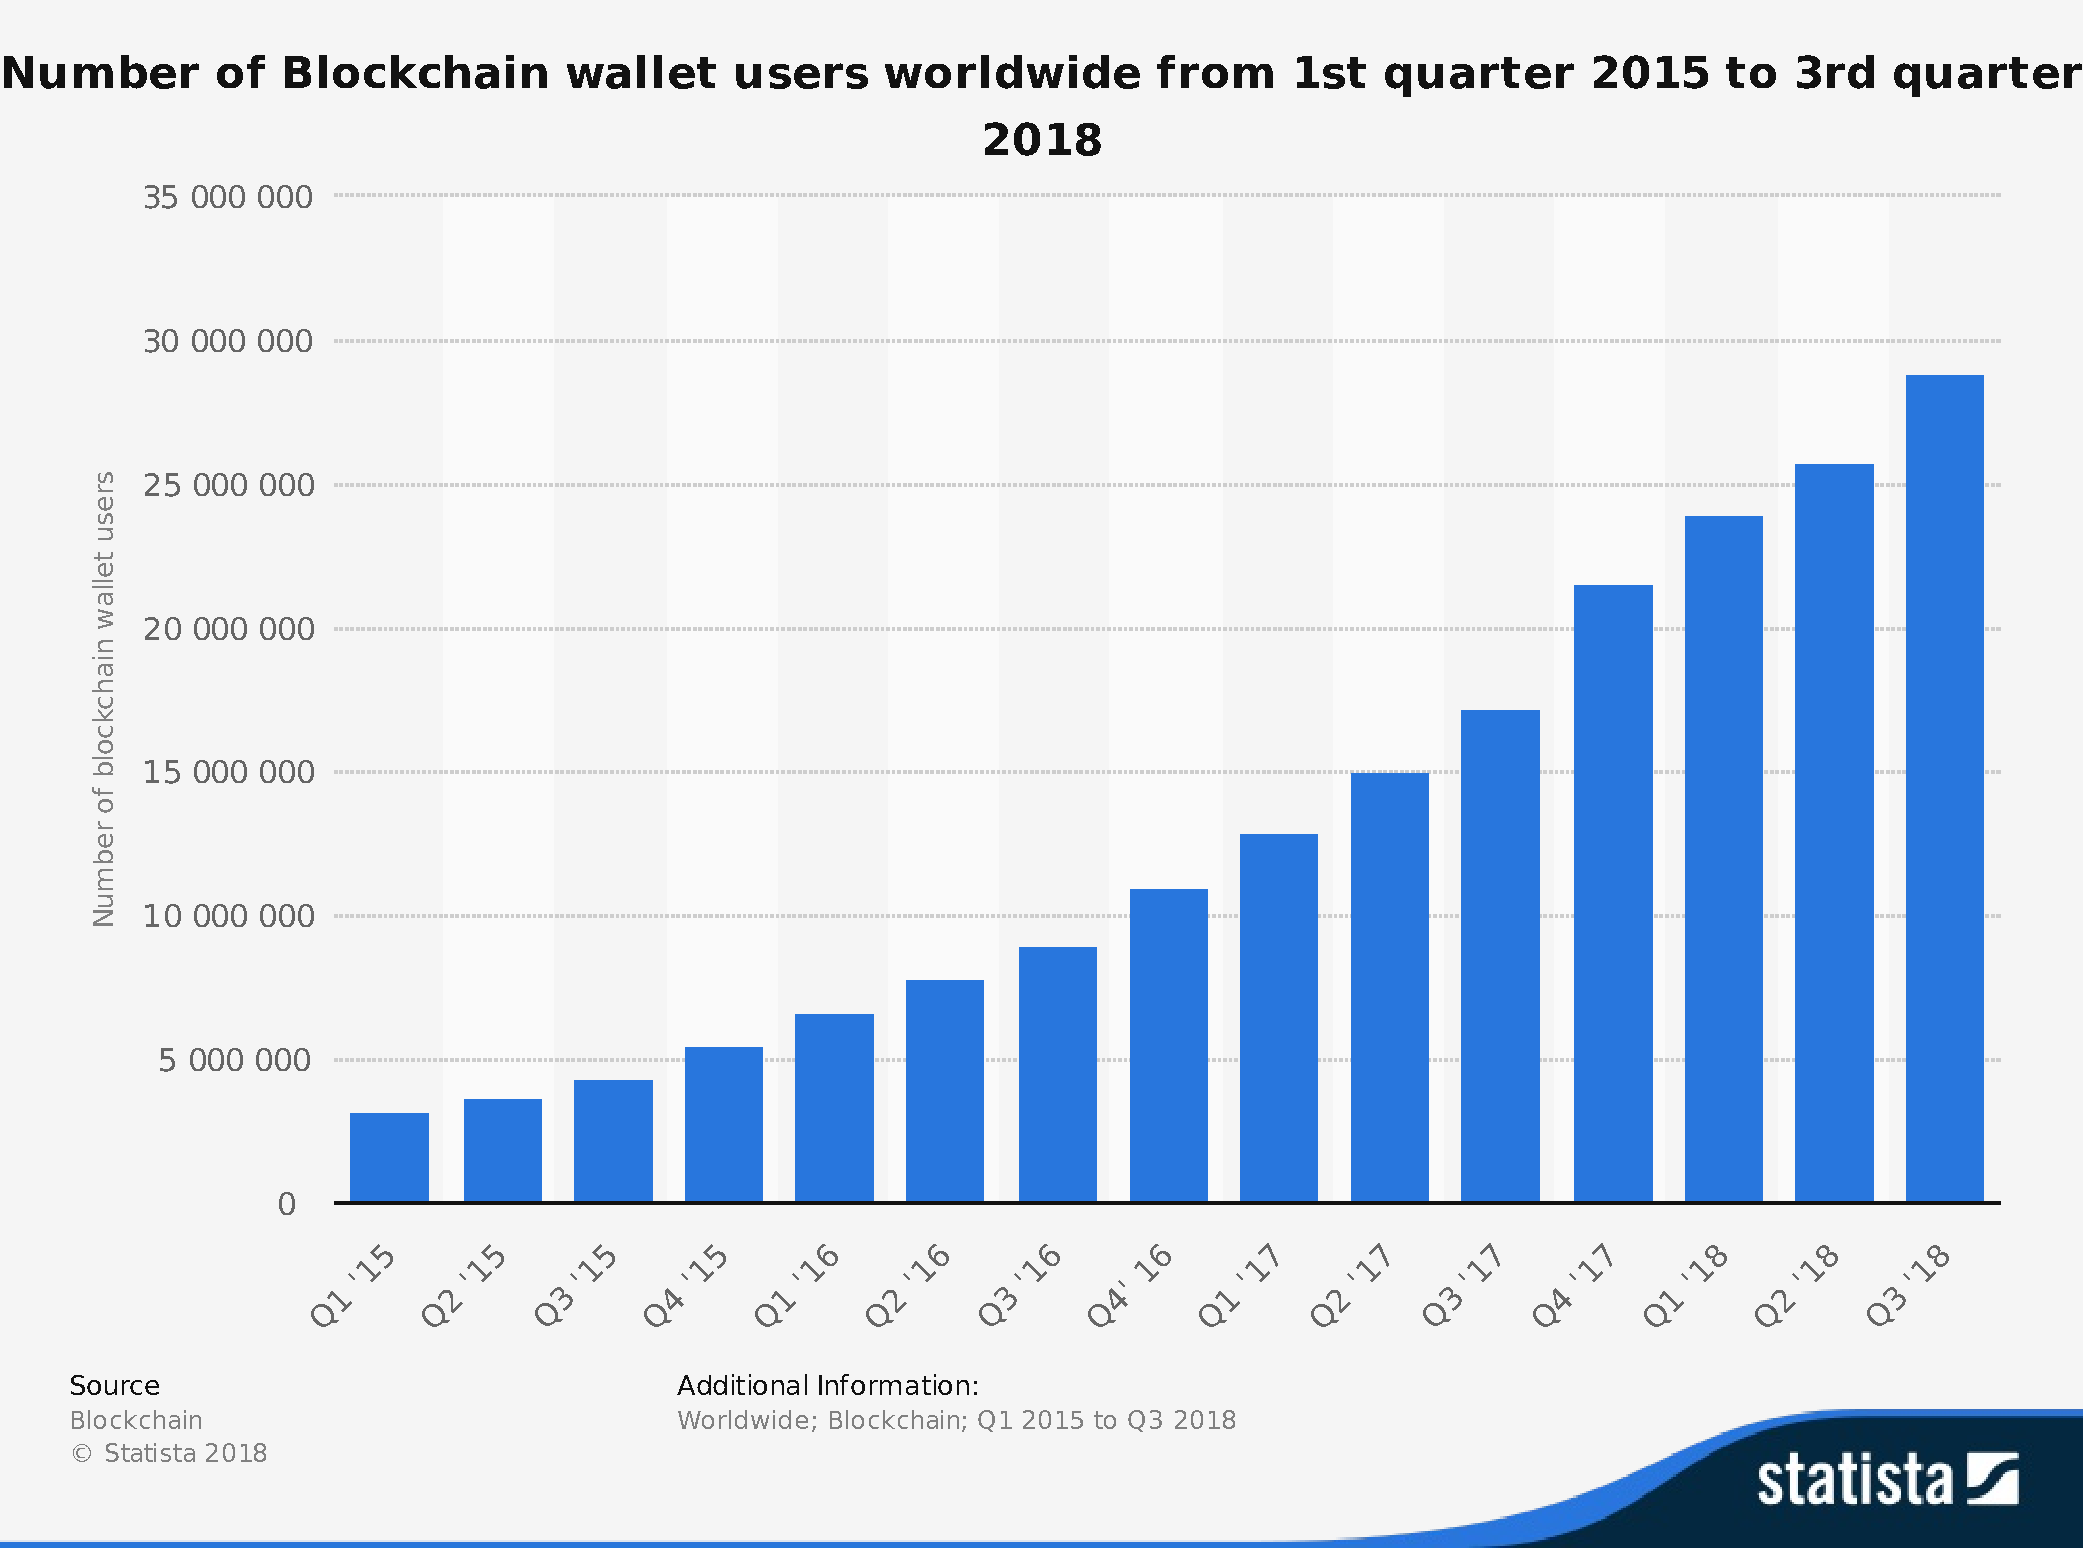
\includegraphics[width=.75\linewidth]{images/chap_intro/number-of-blockchain-wallet.pdf}
	\caption{Numero di portafogli blockchain nel mondo \cite{number-of-blockchain-wallet}}
	\label{fig:number-of-blockchain-wallet}
\end{figure}

In figura \ref{fig:model-focus-for-blockchain}
vediamo i risultati di un sondaggio condotto a livello mondiale da \textit{Deloitte} nell'aprile 2018.
Alla domanda "Su quale modello blockchain stai concentrando le tue attività?"
il 52\% delle organizzazioni intervistate stanno concentrando i propri sforzi hanno risposto con
\textit{blockchain permissioned} \cite{model-focus-for-blockchain}.
\begin{figure}[H]
	\centering
	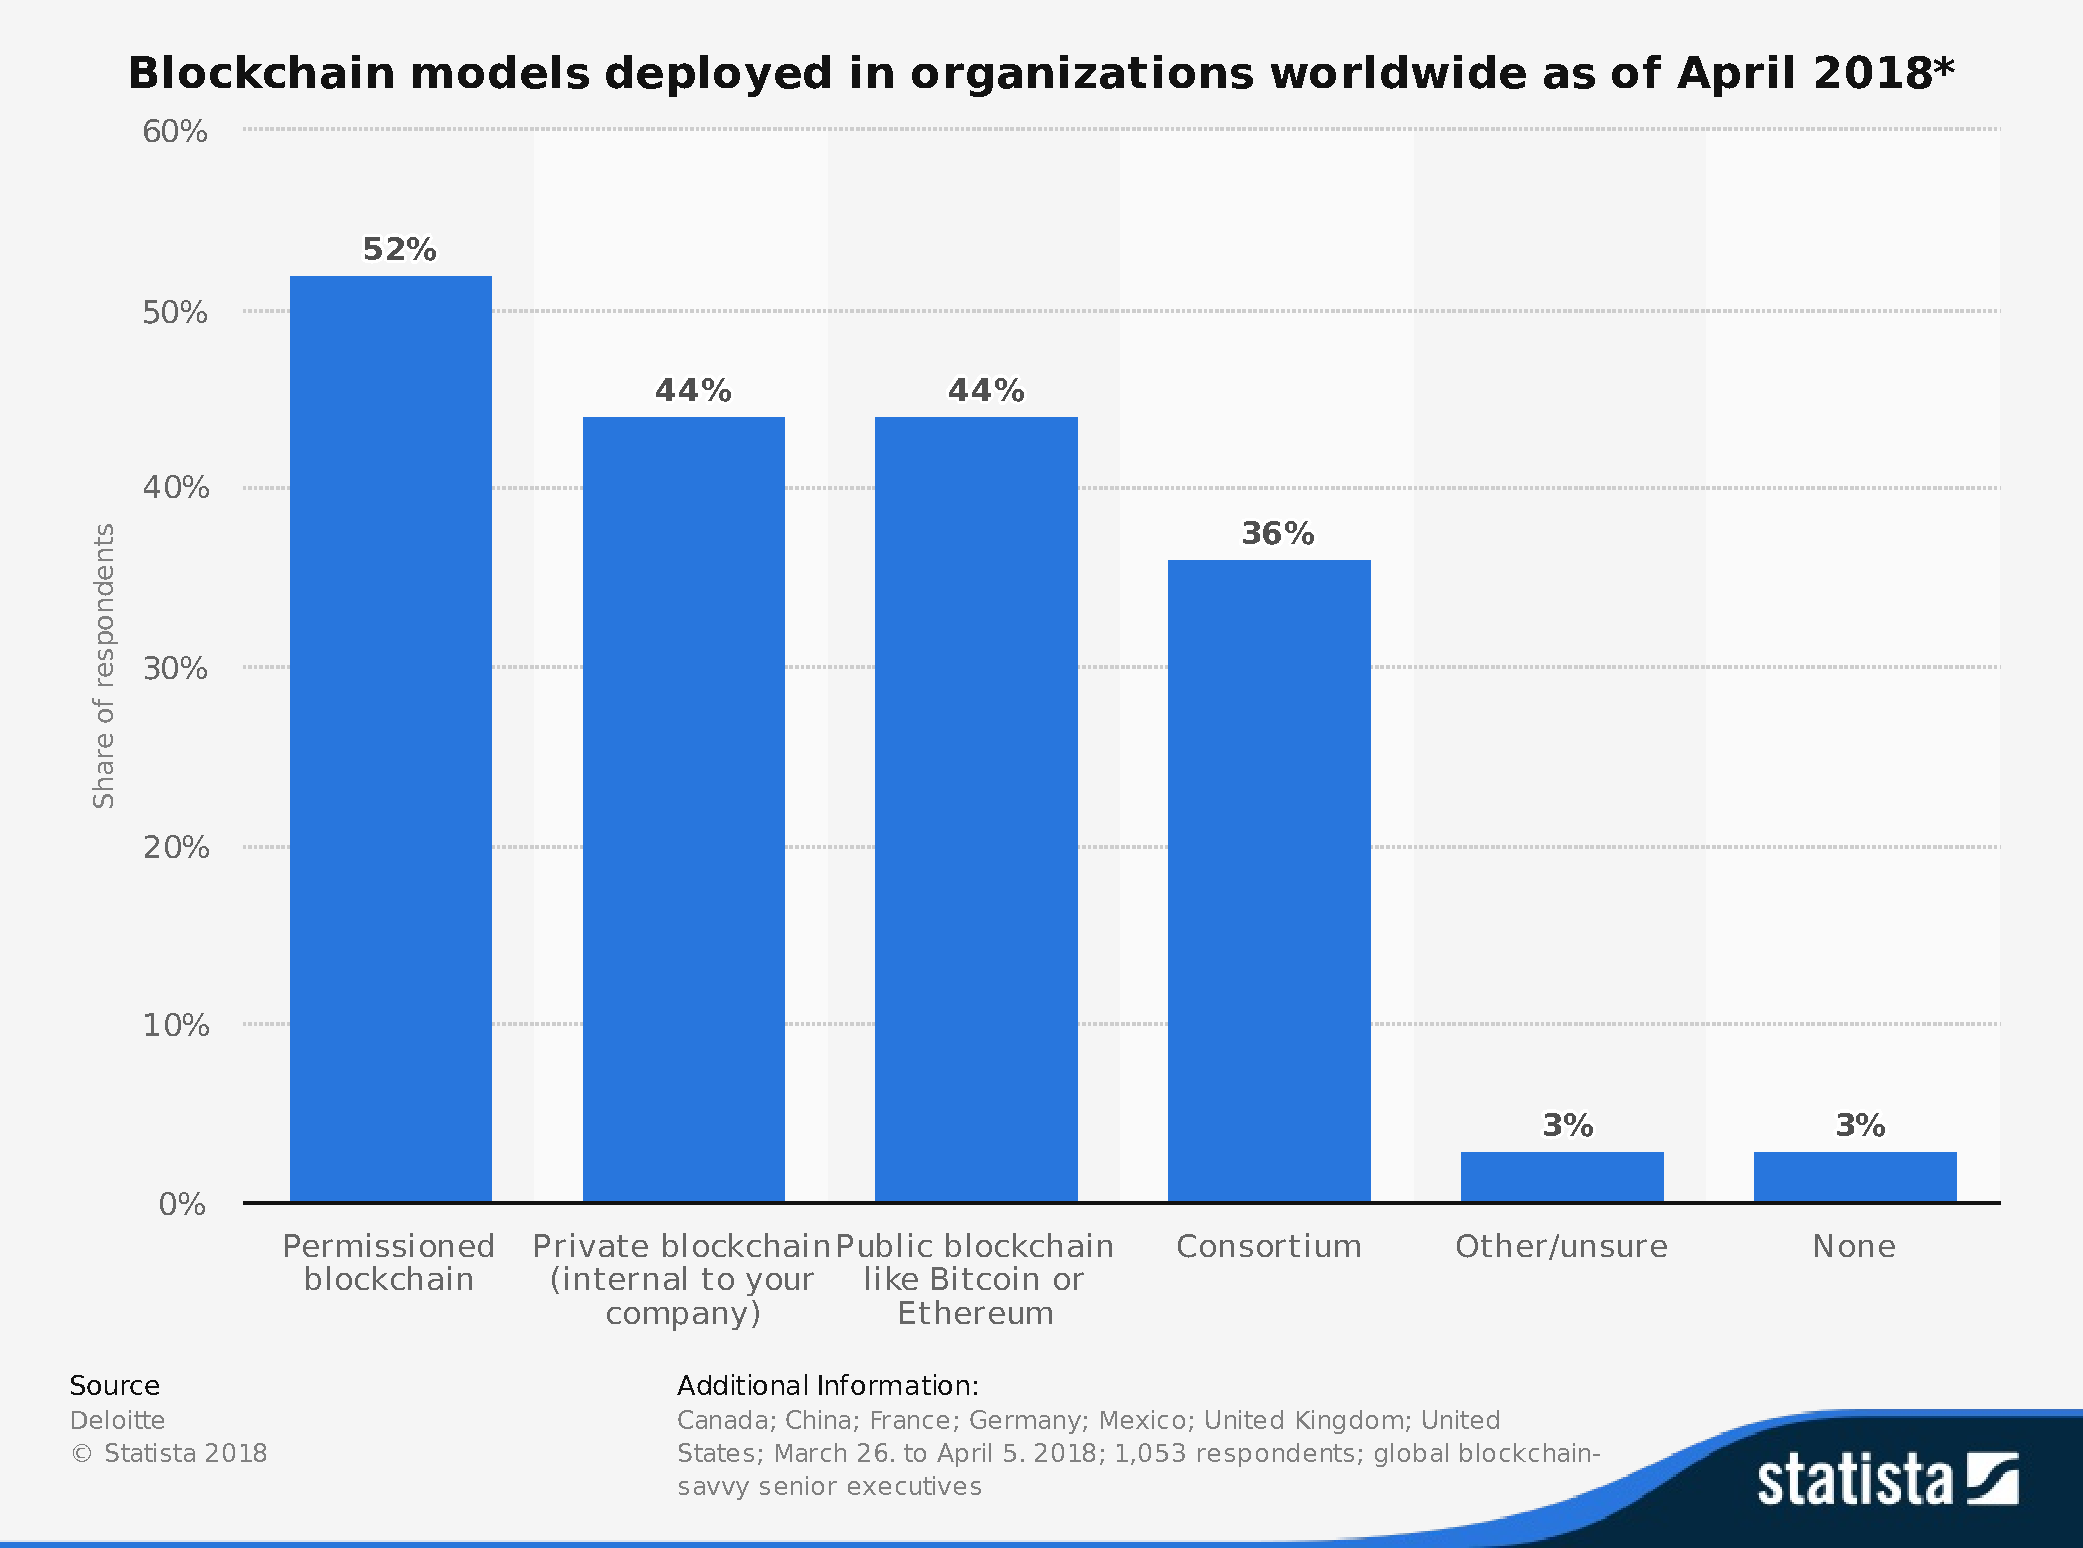
\includegraphics[width=.75\linewidth]{images/chap_intro/model-focus-for-blockchain.pdf}
	\caption{Modelli blockchain utilizzati dalla organizzazioni \cite{model-focus-for-blockchain}}
	\label{fig:model-focus-for-blockchain}
\end{figure}

La blockchain è una tecnologia relativamente giovane. Come è lecito attendersi, le aziende
non hanno ancora maturato una forte esperienza con questa tecnologia, ma ciononostante
sono consapevoli che si tratta
di una opportunità da seguire con attenzione.
Secondo \textit{PwC} solo il 15\% delle aziende U.S.A.
attive nel mondo blockchain sono arrivate ad utilizzare
la blockchain in produzione \cite{stages-of-blockchain-incorporation} e secondo
\textit{eft Supply Chain \& Logistics Business Intelligence}
il 69\% delle organizzazioni intervistate ha dichiarato di stare investendo
nel comprendere la tecnologia \cite{top-spending-in-supply-chain-industry}.


\begin{figure}[H]
	\begin{minipage}{0.48\textwidth}
		\centering
		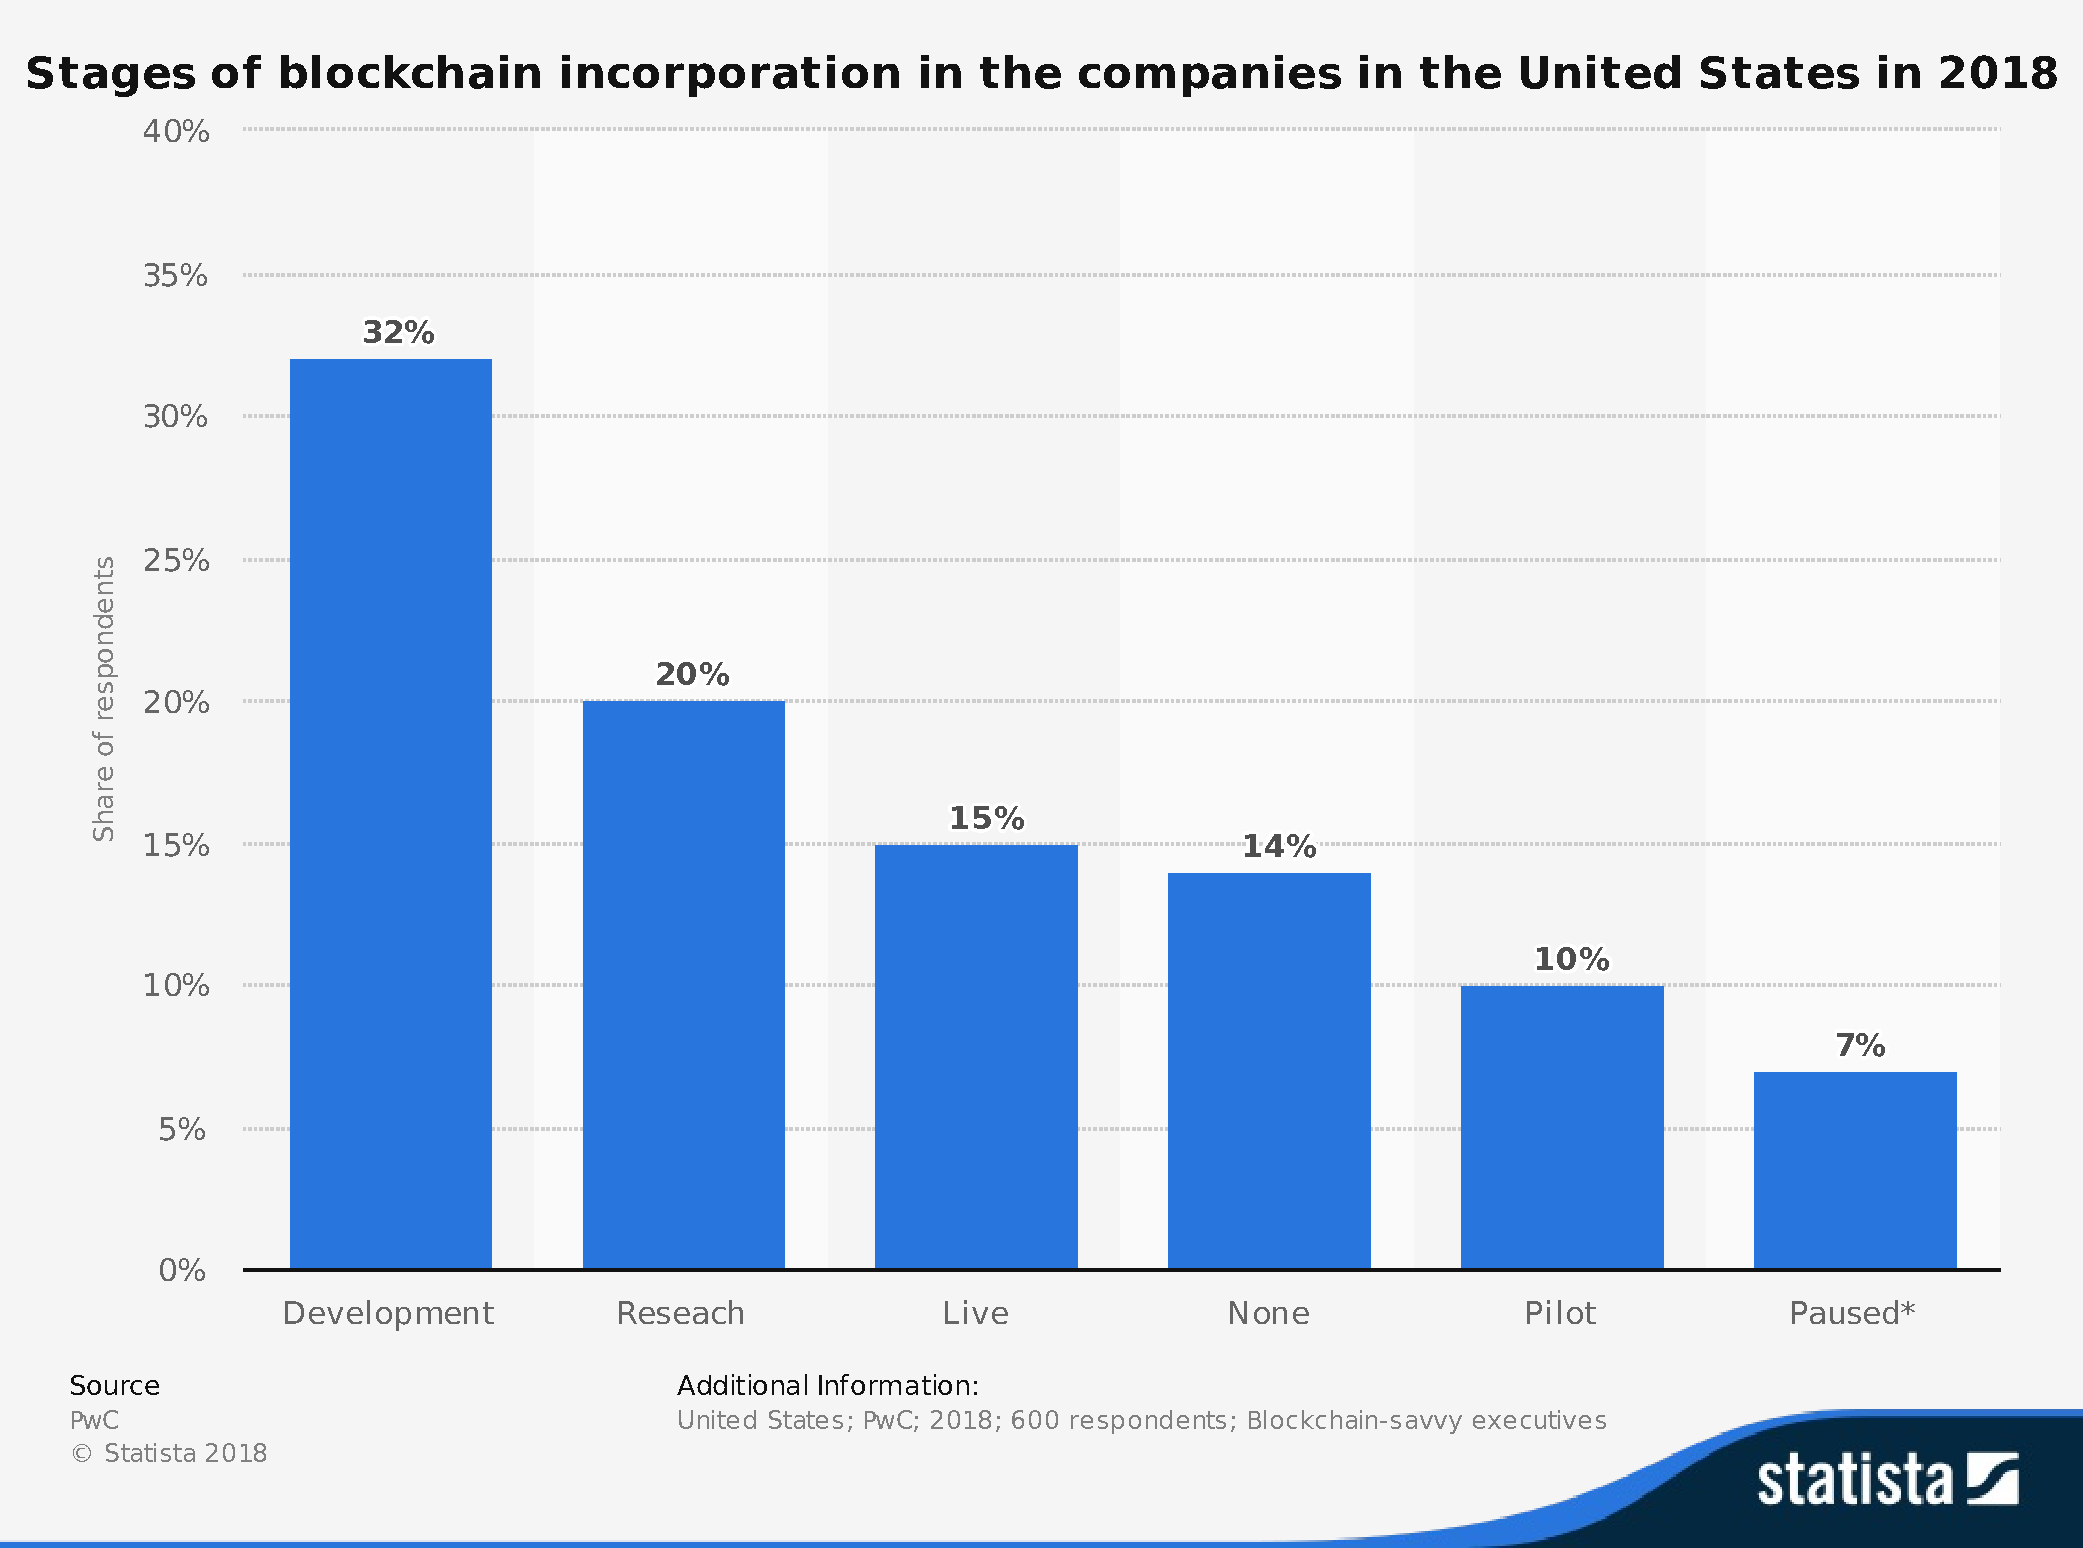
\includegraphics[width=1\linewidth]{images/chap_intro/stages-of-blockchain-incorporation.pdf}
		\caption{Livelli di adozione della blockchain nelle imprese U.S.
			\cite{stages-of-blockchain-incorporation}}
		\label{fig:stages-of-blockchain-incorporation}
	\end{minipage}
	\begin{minipage}{0.48\textwidth}
		\centering
		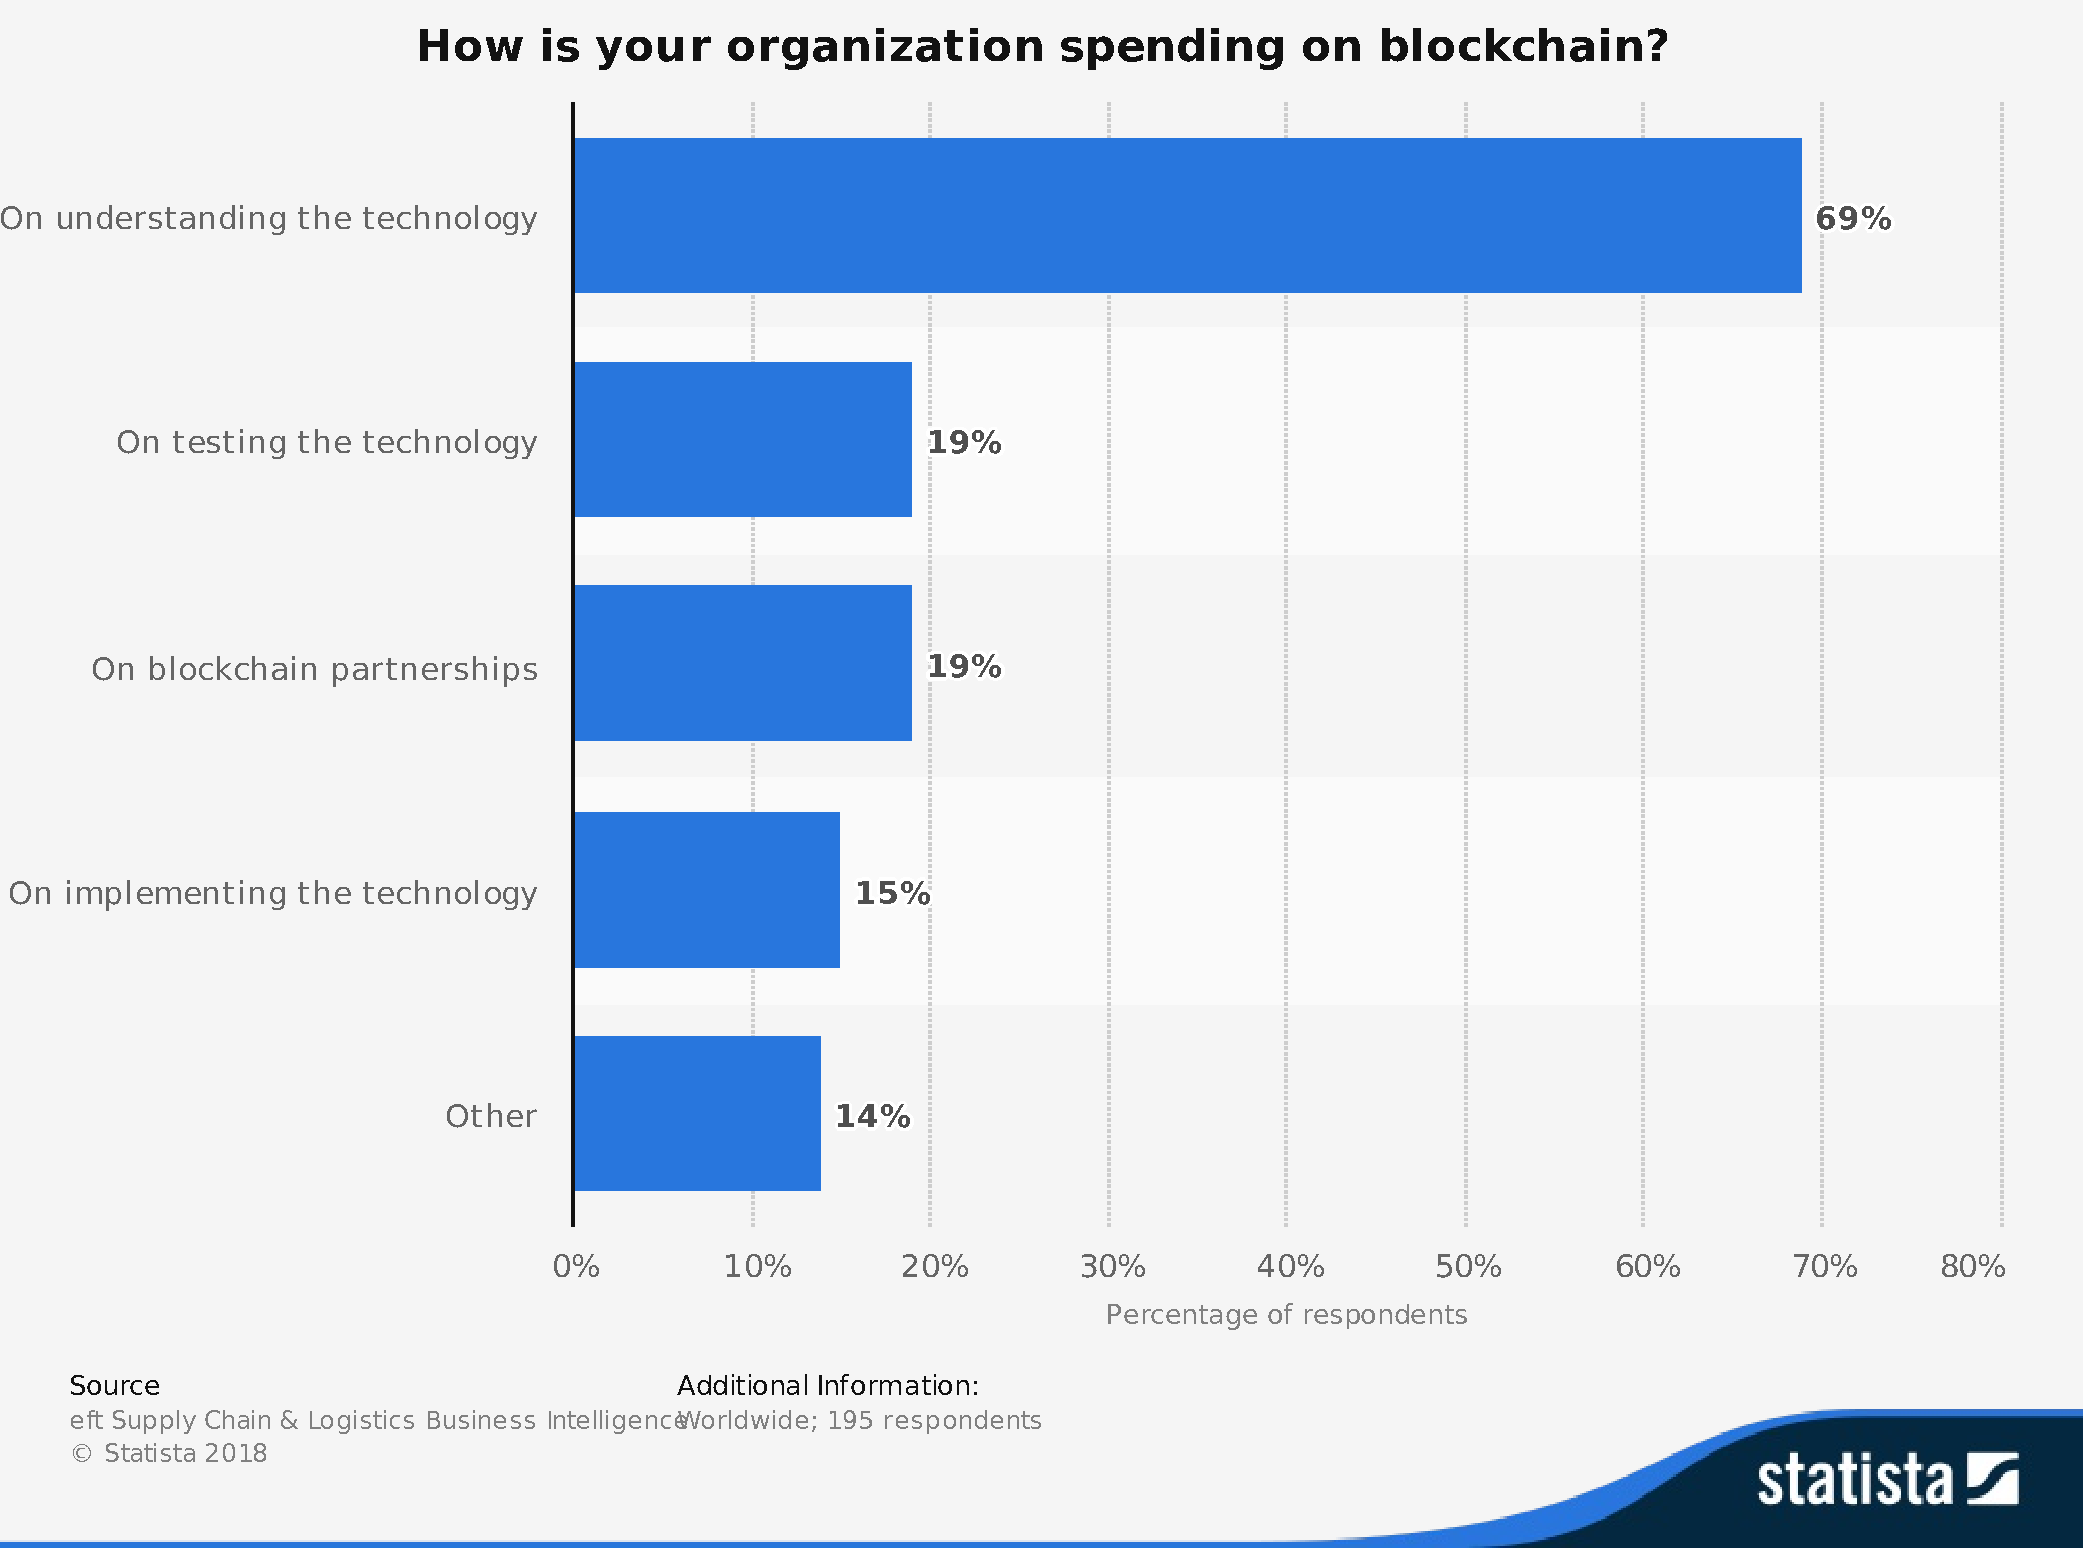
\includegraphics[width=1\linewidth]{images/chap_intro/top-spending-in-supply-chain-industry.pdf}
		\caption{Sondaggio: in che modo la tua organizzazione sta investendo nella blockchain?
			\cite{top-spending-in-supply-chain-industry}}
		\label{fig:top-spending-in-supply-chain-industry}
	\end{minipage}\hfill
\end{figure}

\subsection{L'evozione futura}
In figura \ref{fig:global-blockchain-solutions-spending} viene presentata la spesa complessiva
in soluzioni blockchain suddivisa per macroregioni geografiche tra il 2016 e il 2022.
Nel 2022 la spesa per soluzioni blockchain a livello mondiale toccherà gli 11,65 miliardi di dollari
e nei soli U.S.A viene proiettata a 4,2 miliardi di dollari \cite{global-blockchain-solutions-spending}.
\begin{figure}[H]
	\centering
	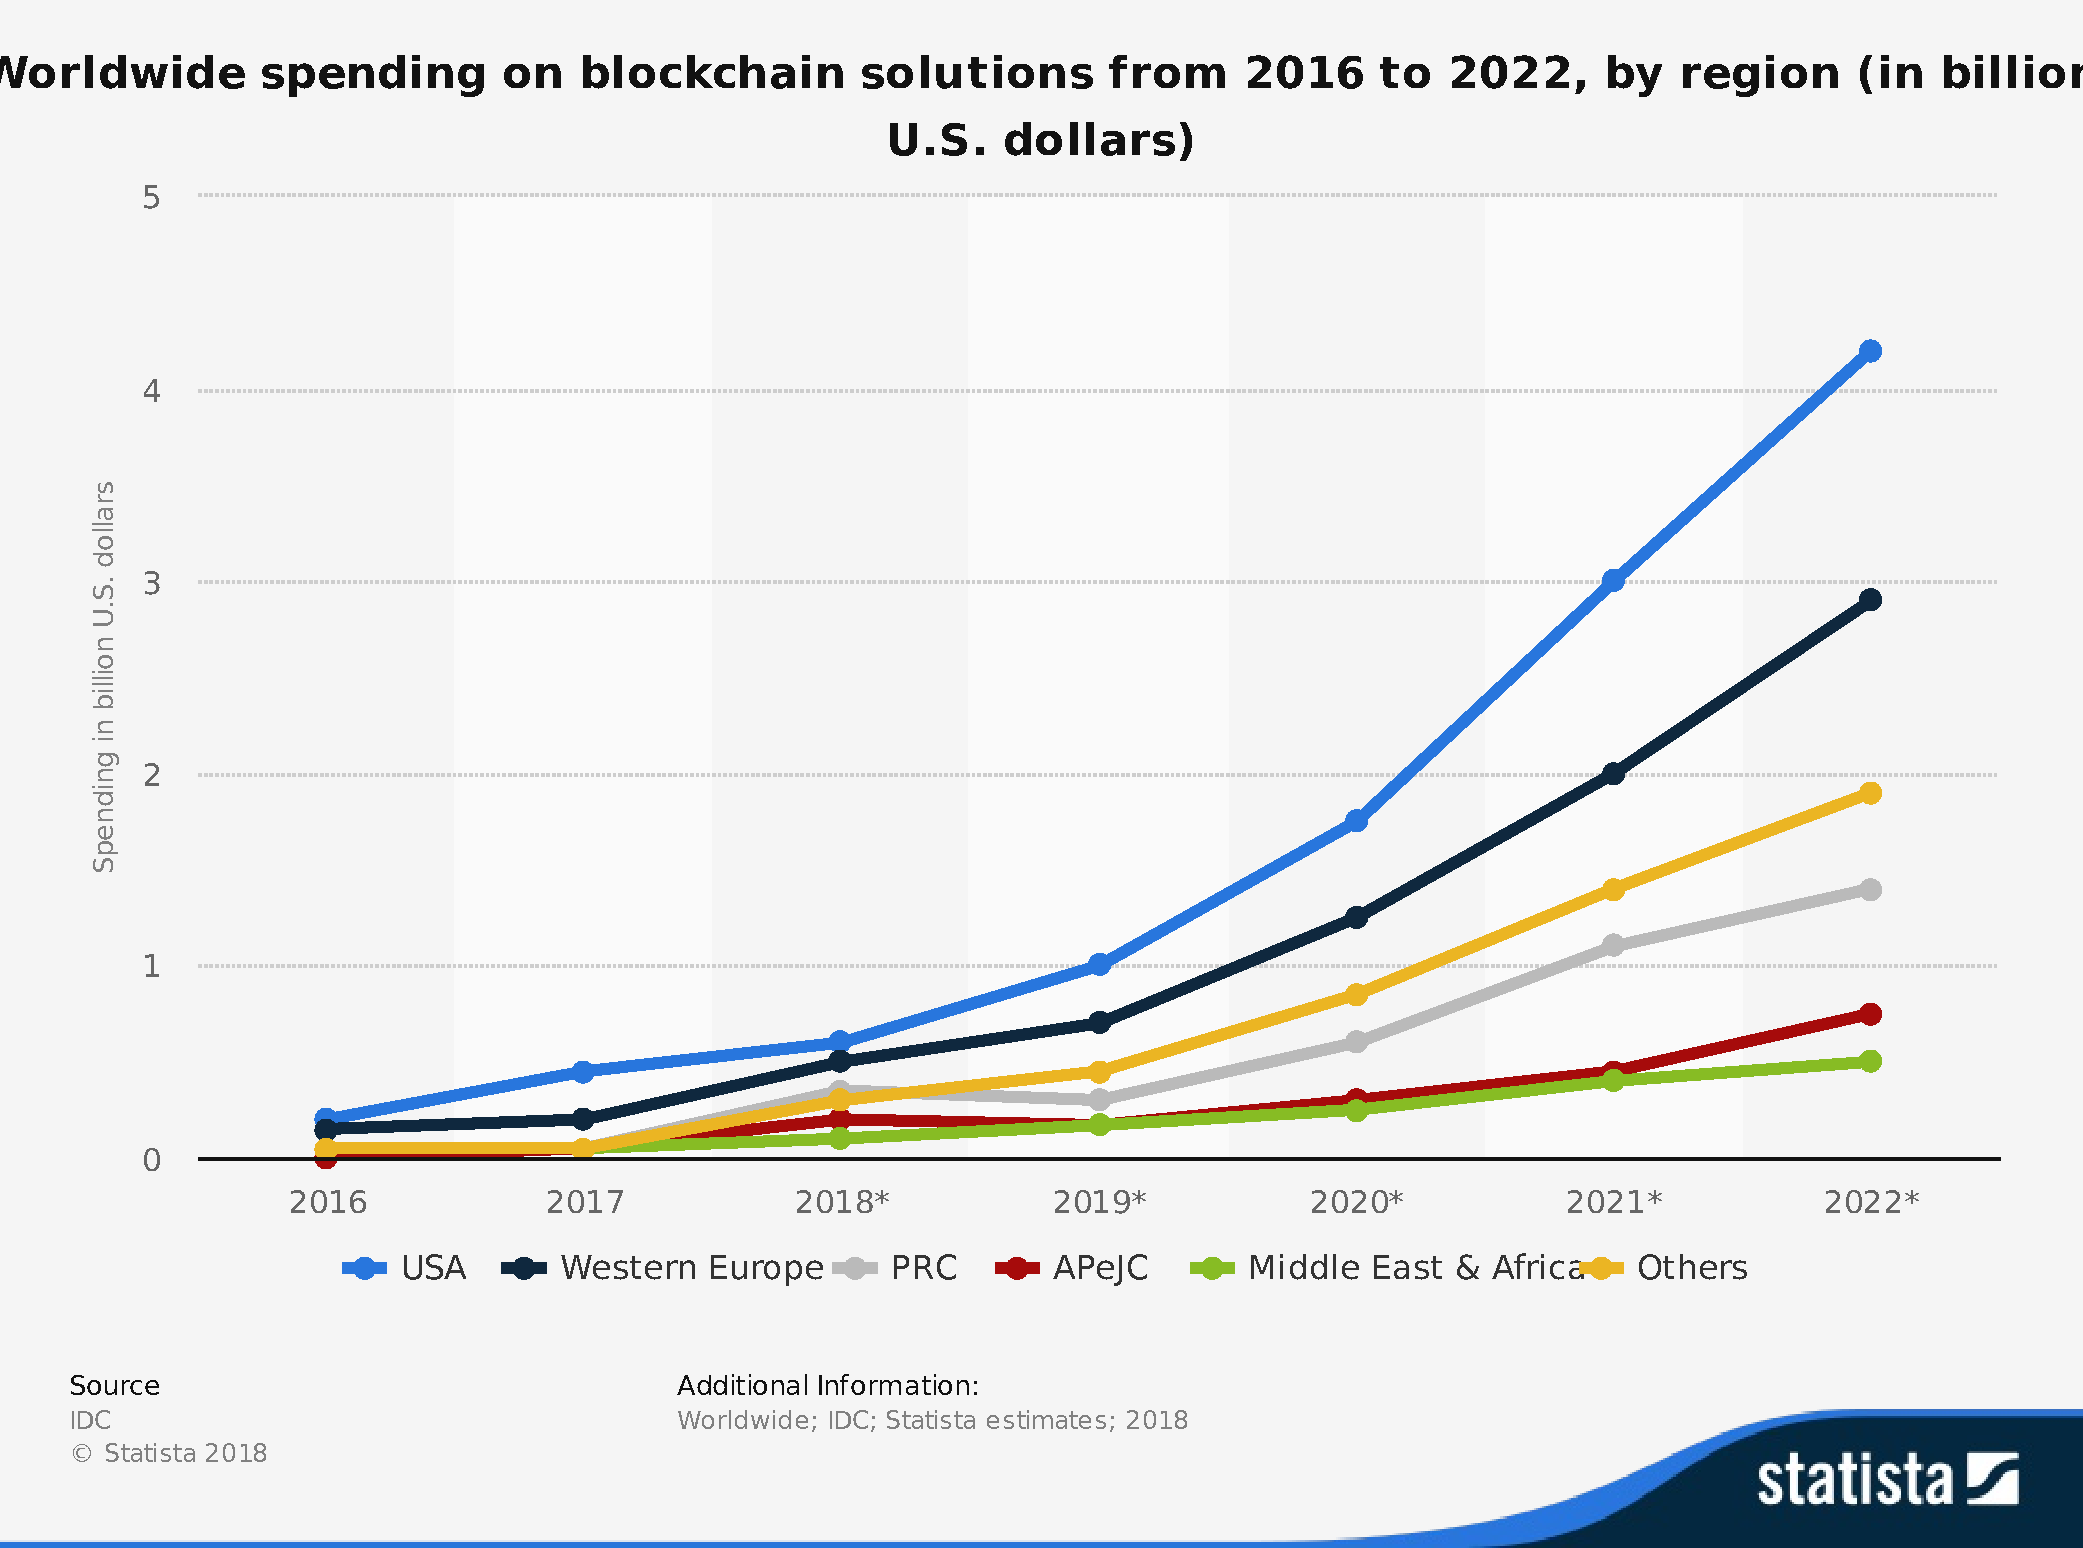
\includegraphics[width=.75\linewidth]{images/chap_intro/global-blockchain-solutions-spending.pdf}
	\caption{Spesa mondiale in soluzioni blockchain per regione (in miliardi di
		dollari U.S.) \cite{global-blockchain-solutions-spending}}
	\label{fig:global-blockchain-solutions-spending}
\end{figure}

In figura \ref{fig:leading-territories-worldwide} vengono mostrati i risultati di un sondaggio
pubblicato in agosto 2018 in cui veniva chiesto
quali sono i territori leader nello sviluppo di tecnologie blockchain.
Circa il 18\% dei partecipanti considera la Cina leader nel 2018.
Alla domanda di considerare quale territorio sarebbe il leader nella tecnologia blockchain
lo sviluppo dal 2021 al 2023, la percentuale di rispondenti che
rispondono alla "Cina" è cresciuta al 30\% \cite{leading-territories-worldwide}.

\begin{figure}[H]
	\centering
	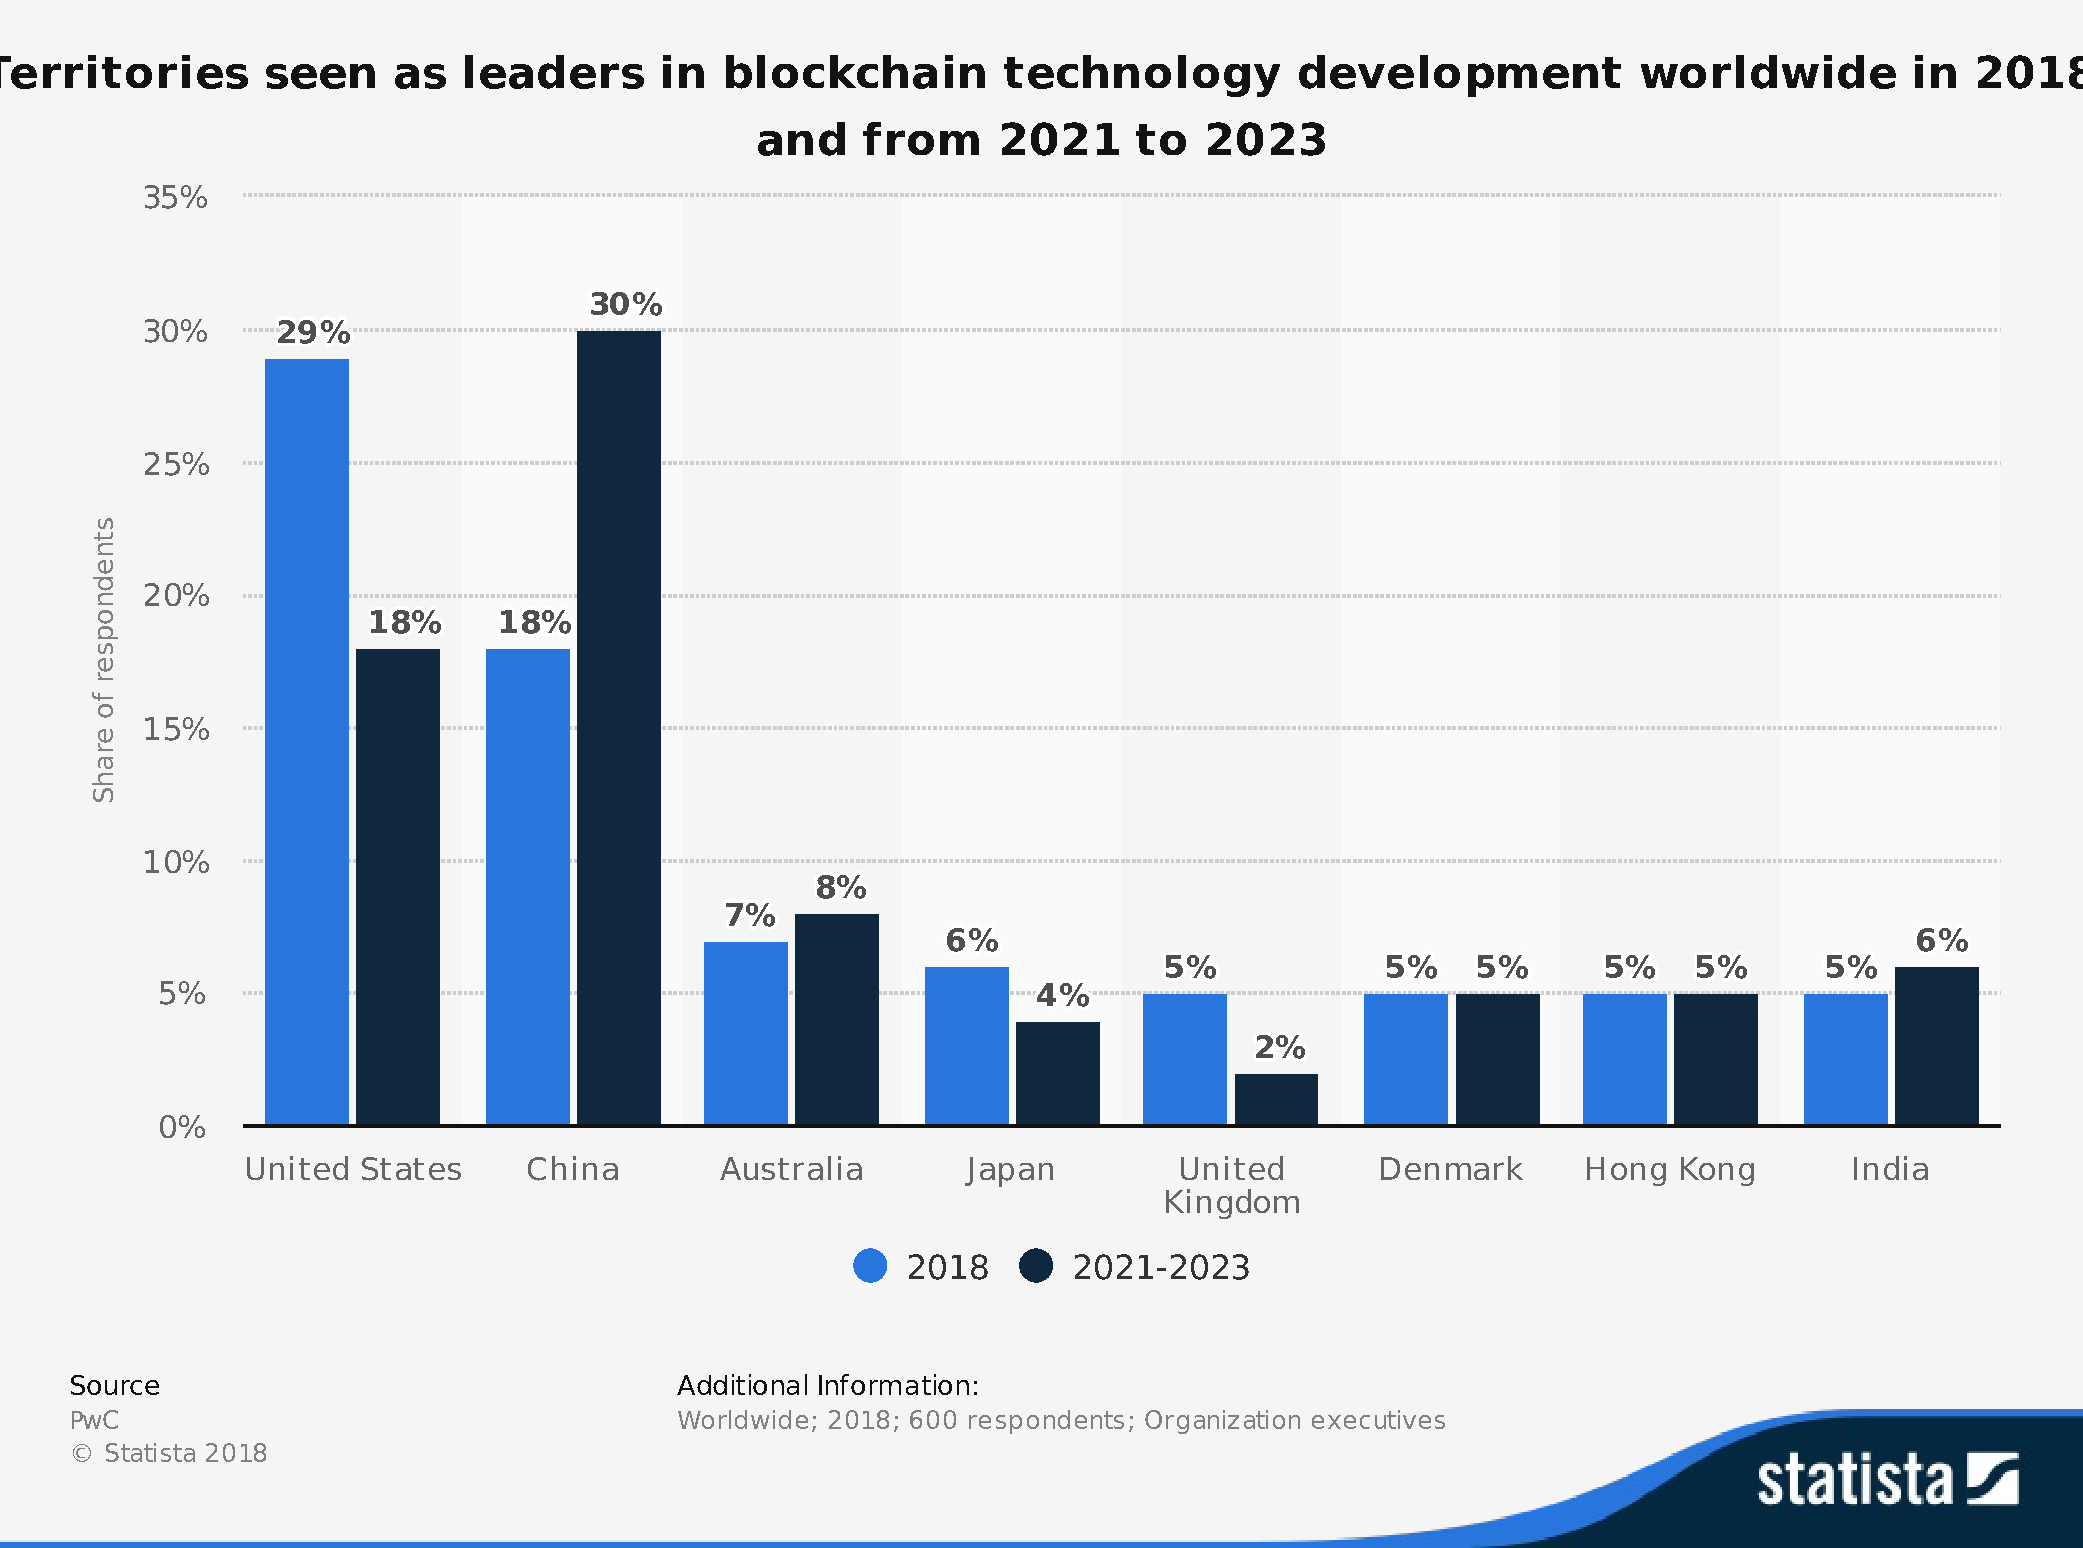
\includegraphics[width=.75\linewidth]{images/chap_intro/leading-territories-worldwide.pdf}
	\caption{Territori mondiali considerati leader nello sviluppo di tecnologie blockchain
		nel 2018 e dal 2021 al 2023
		\cite{leading-territories-worldwide}}
	\label{fig:leading-territories-worldwide}
\end{figure}

\subsection{Le aspettative delle imprese}

Da un sondaggio condotto da \textit{ABN Amro Economisch Bureau} nel 2017 \cite{potential-blockchain-applications}
emerge che secondo i rivenditori olandesi la blockchain può essere uno strumento
utile per velocizzare il proprio business. In particolare,
il 77\% degli intervistati ritiene che possa essere utile per velocizzare
i pagamenti senza utilizzare banche come intermediari e il 58\% crede che
la blockchain possa velocizzare le operazioni logistiche riducendo la burocraziona cartacea
e il coordinamento necessario tra le parti coinvolte.
I risultati del sondaggio sono visibili in figura \ref{fig:potential-blockchain-applications}.
\begin{figure}[H]
	\centering
	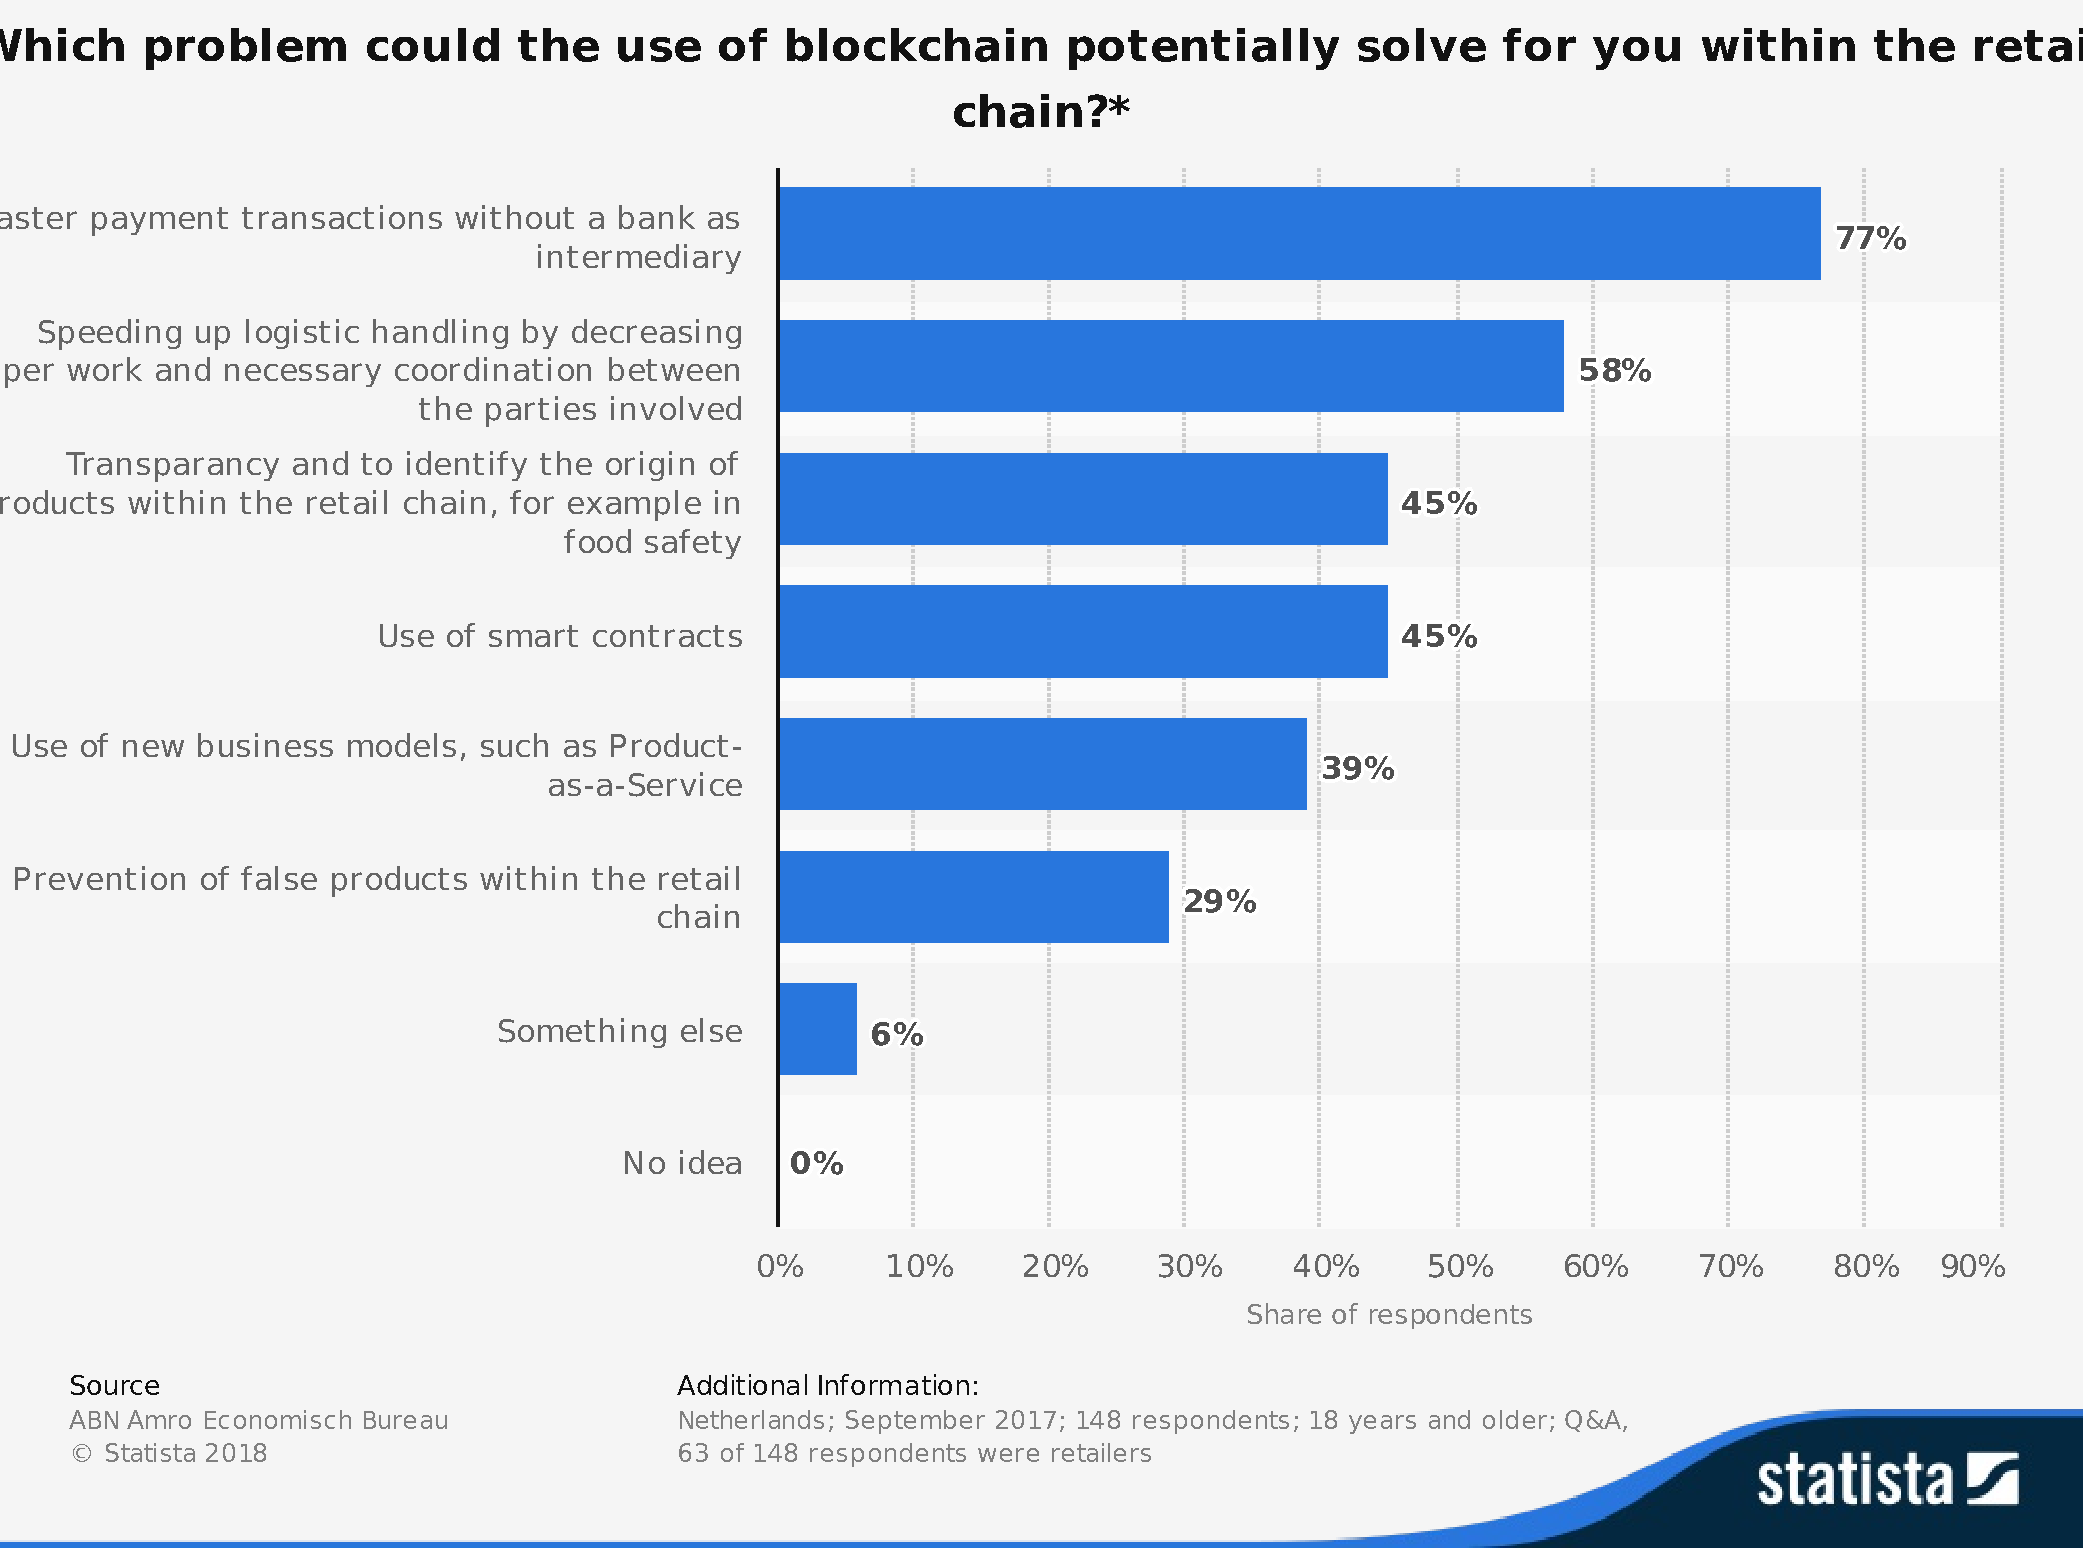
\includegraphics[width=.75\linewidth]{images/chap_intro/potential-blockchain-applications.pdf}
	\caption{Problemi che può potenzialmente risolvere l'uso della blockchain
		nella catena di commercio \cite{potential-blockchain-applications}}
	\label{fig:potential-blockchain-applications}
\end{figure}

In figura \ref{fig:use-cases-among-businesses} vengono esposti i risultati di un sondaggio
condotto tra banche, aziende FinTech e altri istituti finanziari nel 2017 \cite{use-cases-among-businesses}.
L'obiettivo
del sondaggio era quello di individuare quale fossero i casi d'uso di business
della blockchain. È emerso che i più probabili casi d'uso commerciali della blockchain
sono la creazione di una infrastruttura di pagamenti (67\%) e finanza commerciale (61\%).
Da segnalare che il 44\% degli intervistati ha dichiarato che
la tecnologia blockchain può essere utile nella gestione dell'identità digitale.

\begin{figure}[H]
	\centering
	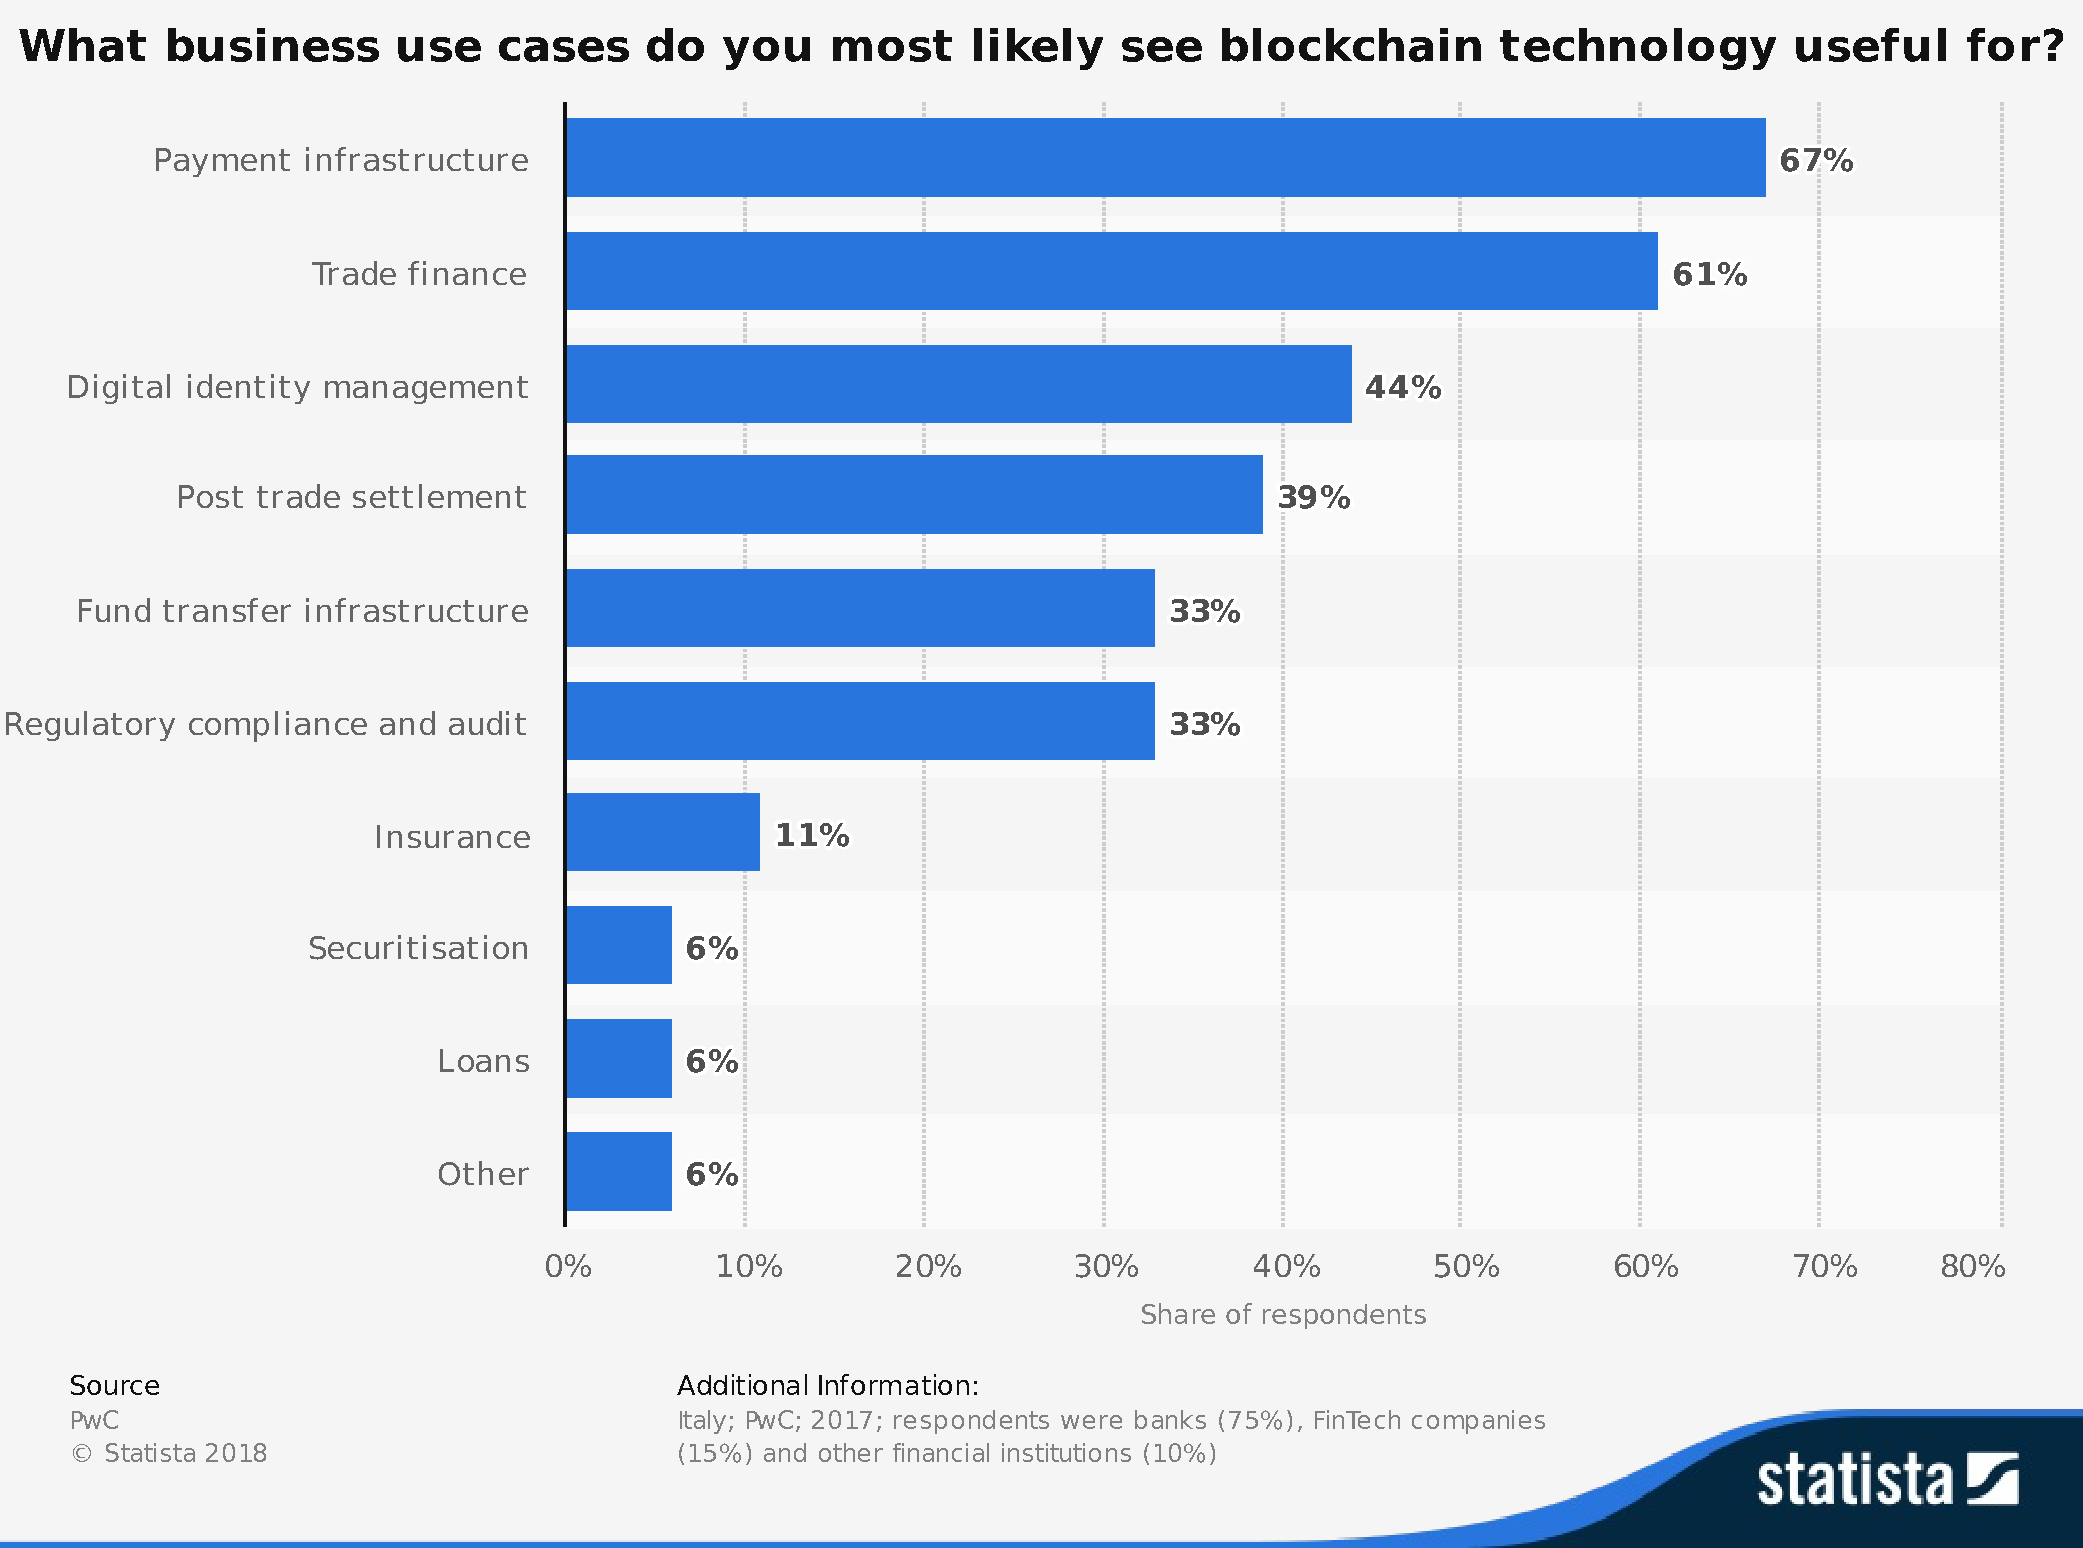
\includegraphics[width=.75\linewidth]{images/chap_intro/use-cases-among-businesses.pdf}
	\caption{Casi d'uso commerciali per la blockchain
		\cite{use-cases-among-businesses}}
	\label{fig:use-cases-among-businesses}
\end{figure}


L'aspetto che nel 2018 rappresenta il principale ostacolo alla adozione della tecnologia blockchain
è l'incertezza normativa. Questo dato emerge dalla statistica condotta da
\textit{PwC} \cite{barriers-worldwide}
e rappresentata in figura \ref{fig:barriers-worldwide}.
Altre barriere rilevanti sono la mancanza di fiducia tra gli utenti e la capacità di riunire la rete.


\begin{figure}[H]
	\centering
	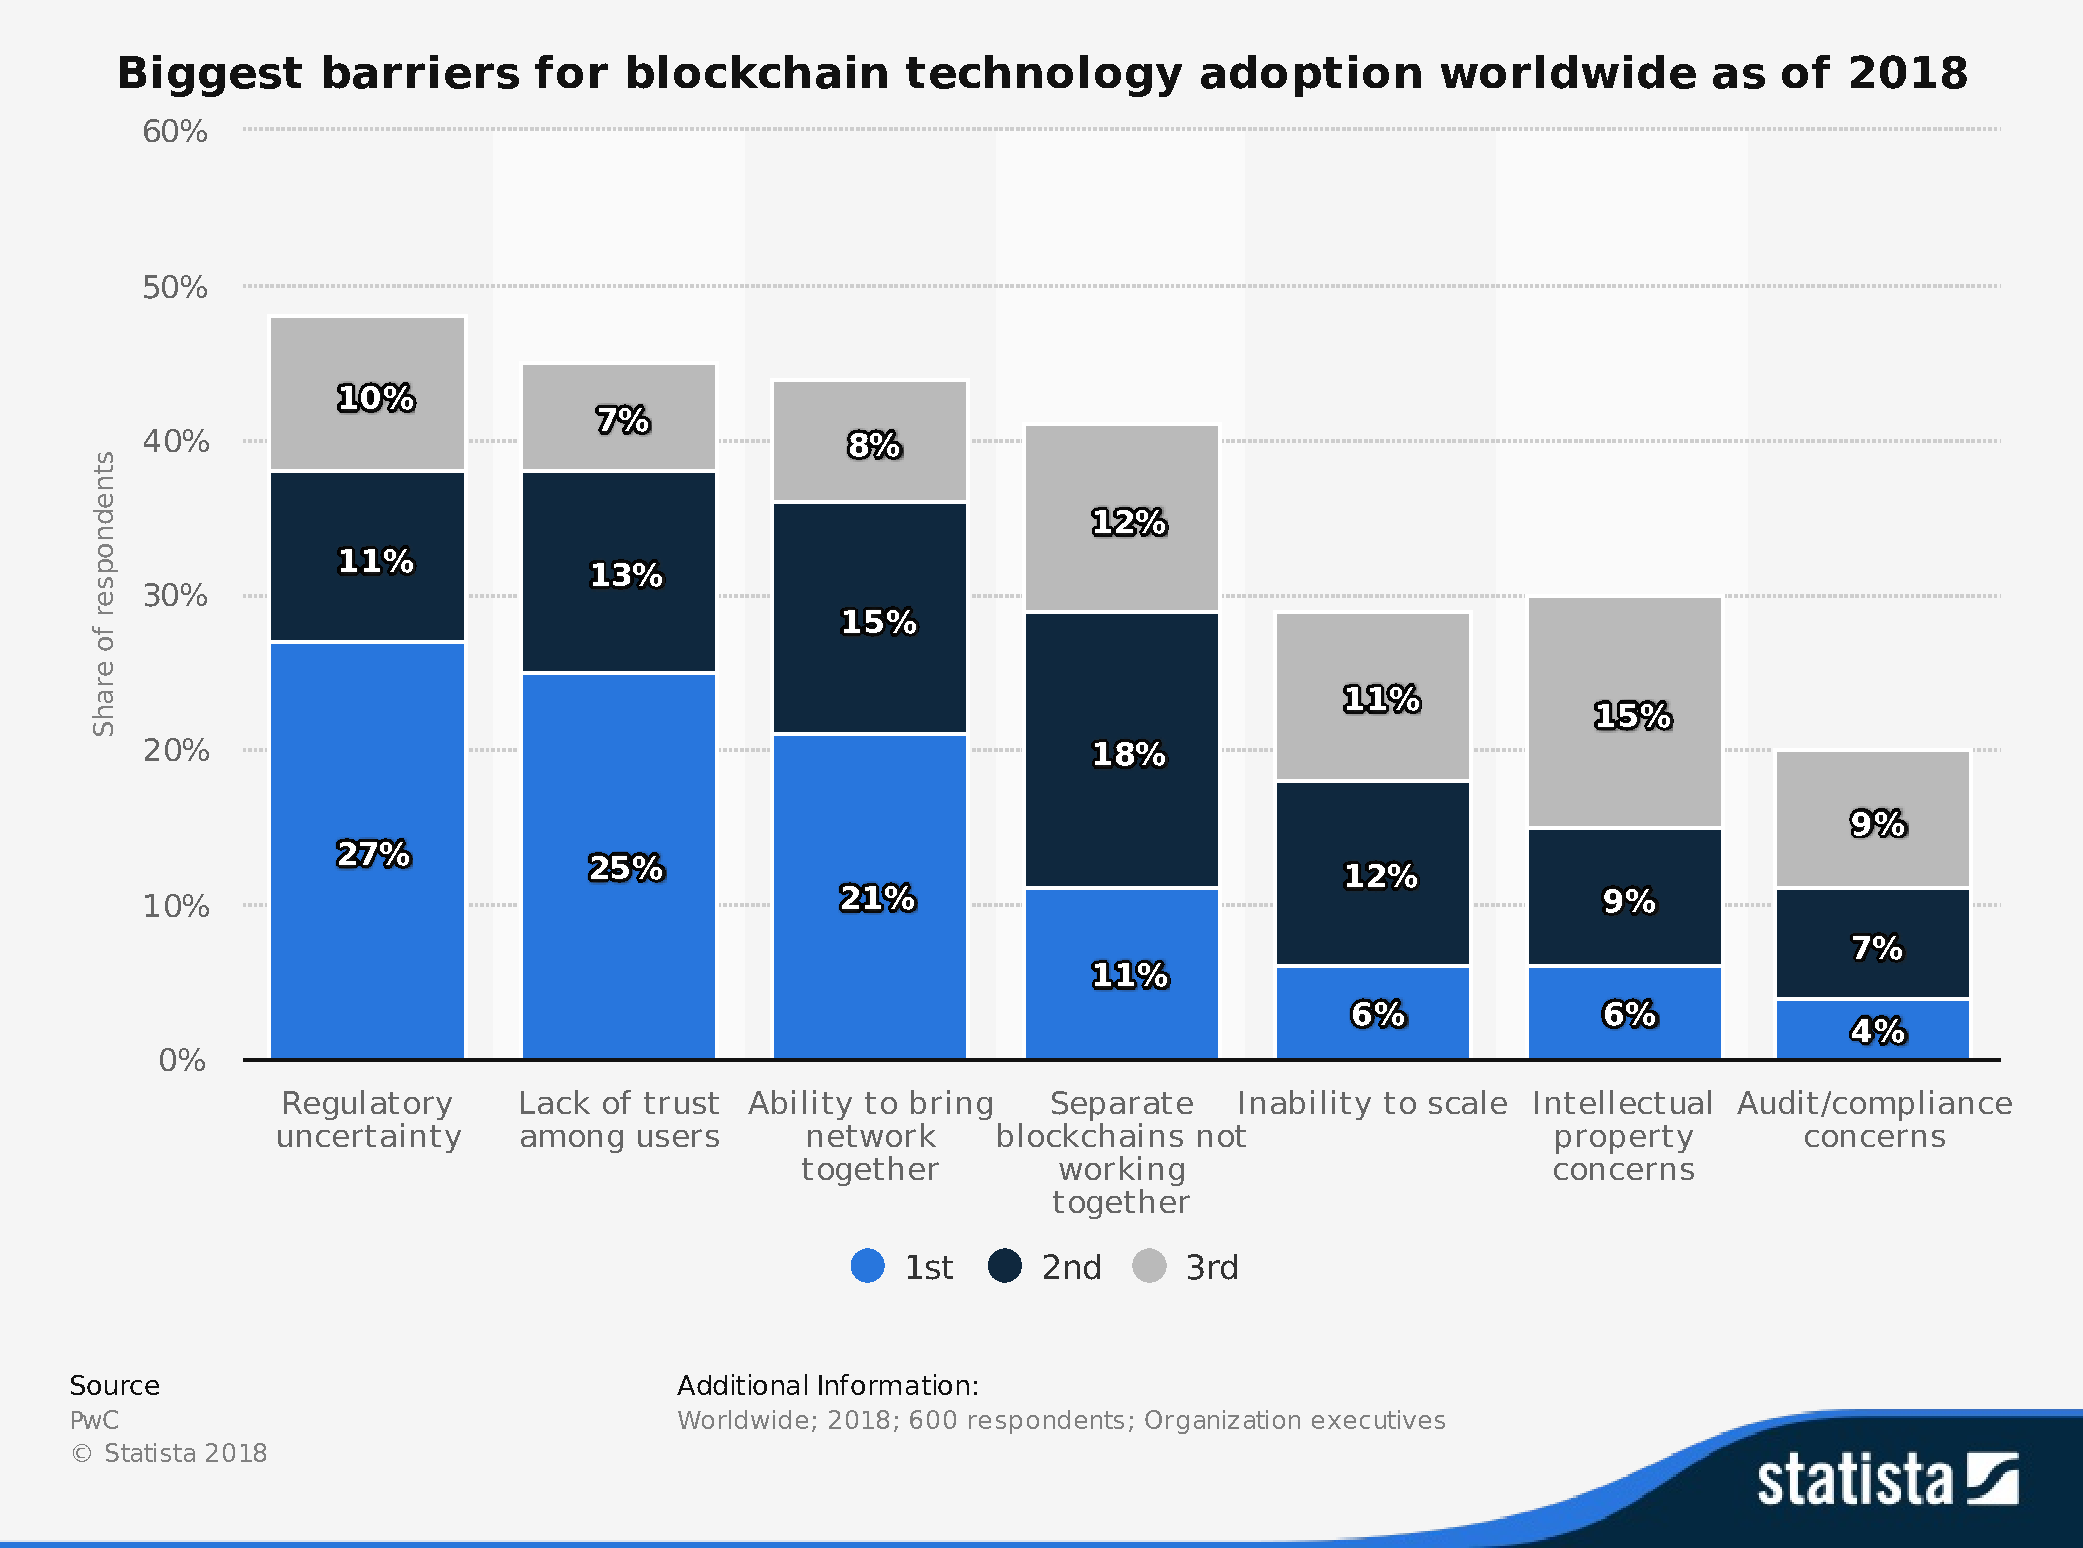
\includegraphics[width=.75\linewidth]{images/chap_intro/barriers-worldwide.pdf}
	\caption{Barriere all'adozione della tecnologia blockchain
		\cite{barriers-worldwide}}
	\label{fig:barriers-worldwide}
\end{figure}